\section{General portrait of homological theories}
A homological theory for a category $\mathcal C$ consist in a sequence of covariant functors $H_n : \mathcal C \longto \Ab{\Grp}$ for each $n\in \N$ which satisfies some set of axioms, which depends on what theory one is interested. For example, if $\mathcal C$ contains a nice homotopical concept, it is rather common to ask for homotopical invariance. Some other axioms are required to obtain long exact sequences in order to deal with short exact sequences. The usual notation is:
\begin{equation*}
    \describefunctor{H_n}{\mathcal{C},A,\phi,B}{\Ab{\Grp},H_n(A),\phi_n,H_n(B)}
\end{equation*}
We also need a way to translate short exact sequences of the form
$$0 \longto A \longto B \longto C \longto 0$$ 
from the original category to higher counterparts obtained by $H_n$, hence, every homology theory seeks to define a connecting morphism $\delta_n : H_n(C) \longto H_{n+1}(A)$ into a long exact sequence: 
\begin{equation*}
    \begin{tikzcd}
  H_0(A) \rar & H_0(B) \rar 
             \ar[draw=none]{d}[name=X, anchor=center]{}
    & H_0(C) \ar[rounded corners,
            to path={ -- ([xshift=2ex]\tikztostart.east)
                      |- (X.center) \tikztonodes
                      -| ([xshift=-2ex]\tikztotarget.west)
                      -- (\tikztotarget)}]{dll}[at end]{\sub\delta0}  \\
  H_1(A) \rar & H_1(C) \rar 
             \ar[draw=none]{d}[name=Y, anchor=center]{}
    & H_1(B) \ar[rounded corners,
            to path={ -- ([xshift=2ex]\tikztostart.east)
                      |- (Y.center) \tikztonodes
                      -| ([xshift=-2ex]\tikztotarget.west)
                      -- (\tikztotarget)}]{dll}[at end]{\sub\delta1} \\ 
    H_2(A) \rar & H_2(B)\rar  & \cdots  \\
\end{tikzcd}
\end{equation*}

On the other hand, as everything containing the prefix ``co'', cohomology theories are consisted of contra-variant functors $(H^n)_{n}$ with the same pay-off. The position of the index on the notation usually indicates what sort of theory one is dealing with. 

Here we are concerned with a homology theory for complex Banach Algebras $\BAlg$ or, more popularly, for $C^*$-algebras $\Cstar$, a.k.a., $K$-theory for Operator Algebras. It is the mirror image of Topological $K$-theory (developed by \textsc{M. F. Atiyah} and \textsc{F. Hirzebruch} \cite{atiyah1959riemann}), in light of \textit{Gelfand Duality} connecting the category of Locally Compact Hausdorff spaces and complex abelian $C^*$-algebras, but not restricted to commutative spaces, which is often referred to as the ``Non-Commutative Topology''. 

%In his work to reformulate Riemman-Roch theorem \cite{borel1958theoreme}, \textit{A. Grothendieck} introduces the group $K(A)$ associated to a subcategory of an abelian category, which nowadays, it is the so called ``Grothendieck's group''. That's where is from the letter $K$, which he had chosen for ``Klassen''. His reformulation famously contains his legendary drawing:
%\begin{figure}[H]
%	\centering
%	% Original artwork by Alexander Grothendieck: the commutative diagram from the
% Grothendieck-Riemann-Roch theorem, surrounded by fire and two devils carrying
% forks.
% Generated with svg2tikz <https://github.com/xyz2tex/svg2tikz> from
% https://en.wikipedia.org/wiki/File:Grothendieck-Riemann-Roch.jpg
% Copyleft Pablo (C) 2021
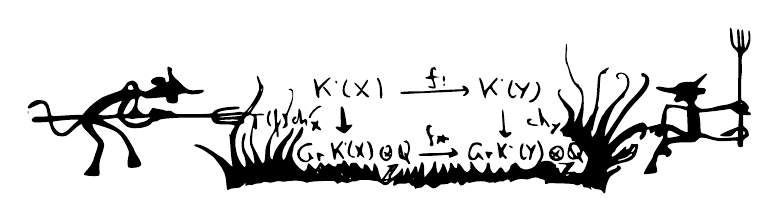
\begin{tikzpicture}[scale=0.45,y=0.80pt, x=0.80pt, yscale=-1, xscale=1, inner sep=0pt, outer sep=0pt]
  \path[fill=black,line width=0.080pt] (705.6108,0.0011) .. controls (705.2593,-0.0223) and (704.9780,0.3330) .. (704.9780,0.8580) .. controls (704.8780,1.5580) and (704.9776,5.0583) .. (705.0776,8.6583) .. controls (705.2776,15.8583) and (706.8781,19.8579) .. (710.5781,22.2579) .. controls (712.5781,23.5579) and (713.0778,24.7586) .. (713.2778,29.9586) .. controls (713.3461,43.0978) and (713.1607,57.2962) .. (713.1006,67.8512) -- (712.9995,73.1510) -- (708.3999,75.1520) .. controls (705.8999,76.2520) and (701.8007,77.4510) .. (699.2007,77.6510) .. controls (696.6007,77.9510) and (692.2997,78.8520) .. (689.6997,79.6520) .. controls (687.0997,80.5520) and (682.4996,81.3512) .. (679.5996,81.3512) .. controls (675.1996,81.5512) and (673.8997,81.1514) .. (671.6997,79.0514) .. controls (668.6997,76.2514) and (668.2000,73.5515) .. (670.5000,72.6515) .. controls (671.3000,72.3515) and (672.0000,70.9519) .. (672.0000,69.5519) .. controls (672.0000,67.3519) and (672.3999,67.0514) .. (675.3999,67.0514) .. controls (679.0999,67.0514) and (681.3993,65.1522) .. (680.7993,62.3522) .. controls (680.4993,60.9522) and (679.4997,60.5519) .. (676.1997,60.5519) .. controls (673.8997,60.5519) and (672.0000,60.1510) .. (672.0000,59.6510) .. controls (672.0000,59.1510) and (674.2995,56.1523) .. (676.9995,52.9523) .. controls (679.7995,49.7523) and (682.0005,46.9520) .. (682.0005,46.6520) .. controls (682.0005,45.1520) and (679.4994,46.4514) .. (674.3994,50.5514) .. controls (669.3994,54.6514) and (668.5995,55.0523) .. (664.9995,54.4523) .. controls (659.8995,53.6523) and (652.1995,55.6514) .. (651.4995,58.0514) .. controls (650.7995,60.3514) and (644.6993,61.0510) .. (637.2993,59.6510) .. controls (633.3993,58.9510) and (631.5998,59.0517) .. (630.7998,59.8517) .. controls (629.2998,61.3517) and (635.0004,63.8511) .. (643.4004,65.2511) .. controls (651.8004,66.6511) and (652.5006,67.1511) .. (650.1006,69.7511) .. controls (648.4006,71.5511) and (648.3004,72.1520) .. (649.4004,73.6520) .. controls (650.6004,75.2520) and (651.0994,75.3519) .. (654.8994,74.0519) .. controls (658.7994,72.7519) and (659.1997,72.8521) .. (661.1997,74.7521) .. controls (664.2997,77.9521) and (663.0003,80.2518) .. (658.8003,78.9518) .. controls (657.0003,78.4518) and (652.2007,77.7518) .. (648.2007,77.4518) -- (640.8999,76.9523) -- (639.0000,81.3512) .. controls (637.9000,83.7512) and (636.7003,88.1510) .. (636.3003,91.1510) -- (635.5005,96.4523) -- (628.8003,98.1515) -- (622.1001,99.8522) -- (620.5005,97.4513) .. controls (619.7005,96.1513) and (618.1006,95.0519) .. (617.1006,95.0519) .. controls (614.7006,95.0519) and (604.7001,99.6510) .. (599.6001,103.1510) .. controls (595.7001,105.7510) and (593.6001,107.4523) .. (586.1001,114.4523) -- (582.7002,117.5519) -- (583.4004,114.8522) .. controls (584.0004,112.2522) and (586.6007,107.6514) .. (594.2007,95.5514) .. controls (600.5007,85.5514) and (604.2007,80.8523) .. (613.7007,70.9523) .. controls (621.2007,63.0523) and (624.0000,58.2515) .. (624.0000,53.1515) .. controls (624.0000,49.8515) and (621.5003,46.5519) .. (618.3003,45.5519) .. controls (616.4003,45.0519) and (616.0005,45.3523) .. (616.0005,46.9523) .. controls (616.0005,48.1523) and (616.3003,48.9518) .. (616.8003,48.9518) .. controls (621.1003,48.2518) and (621.1003,53.0510) .. (616.8003,59.6510) .. controls (615.0003,62.3510) and (610.5994,67.4519) .. (606.8994,71.0519) .. controls (603.2994,74.6519) and (598.4998,80.4509) .. (596.2998,84.0509) .. controls (594.0998,87.6509) and (590.7994,92.7522) .. (588.8994,95.3522) .. controls (586.9994,98.0522) and (585.1005,100.9513) .. (584.5005,101.9513) .. controls (584.0005,102.8513) and (582.4998,104.9509) .. (581.2998,106.5509) -- (579.0000,109.5509) -- (579.6006,104.5514) .. controls (580.4006,97.1514) and (586.5005,81.9515) .. (590.5005,77.1515) .. controls (593.4005,73.6515) and (597.3997,70.0514) .. (598.1997,70.0514) .. controls (598.6997,70.0514) and (598.9995,69.3514) .. (598.9995,68.5514) .. controls (598.9995,67.6514) and (599.9005,65.7521) .. (601.0005,64.2521) .. controls (606.9005,56.3521) and (603.6000,45.0509) .. (595.5000,45.0509) .. controls (591.2000,45.0509) and (589.1006,47.9514) .. (591.6006,50.5514) .. controls (592.5006,51.4514) and (593.4993,51.8519) .. (593.7993,51.5519) .. controls (594.1993,51.2519) and (593.9002,50.5515) .. (593.2002,50.1515) .. controls (591.0002,48.8515) and (593.0006,46.0514) .. (596.1006,46.0514) .. controls (601.2006,46.0514) and (603.7995,54.7514) .. (600.4995,61.0514) .. controls (599.6995,62.6514) and (594.5005,68.4523) .. (589.0005,73.9523) .. controls (583.5005,79.3523) and (579.0000,84.5517) .. (579.0000,85.3517) .. controls (579.0000,86.2517) and (578.4999,87.0516) .. (577.8999,87.2516) .. controls (576.6999,87.6516) and (573.9004,94.0520) .. (571.4004,102.1520) .. controls (570.0004,106.9520) and (565.9995,111.8522) .. (565.9995,108.8522) .. controls (565.9995,107.9522) and (565.8000,105.7523) .. (565.5000,103.9523) .. controls (565.1000,101.2523) and (565.2003,101.0514) .. (565.8003,103.0514) .. controls (566.5003,105.0514) and (566.9004,103.8519) .. (568.4004,96.5519) .. controls (569.4004,91.5519) and (570.9995,85.6511) .. (571.9995,83.2511) .. controls (573.0995,80.9511) and (573.5000,79.2509) .. (573.0000,79.5509) .. controls (571.8000,80.3509) and (571.8000,79.3517) .. (573.0000,73.3517) .. controls (573.5000,70.7517) and (574.0993,63.9513) .. (574.2993,58.4513) .. controls (574.4993,52.8513) and (574.9994,47.7515) .. (575.3994,47.1515) .. controls (575.7994,46.5515) and (577.2001,46.0514) .. (578.6001,46.0514) .. controls (580.0001,46.0514) and (580.9000,45.6520) .. (580.5000,45.1520) .. controls (580.2000,44.5520) and (581.0007,43.2520) .. (582.2007,42.1520) .. controls (585.7007,38.8520) and (581.9997,39.5514) .. (577.1997,43.0514) .. controls (572.4997,46.3514) and (572.3996,46.9509) .. (571.5996,63.0509) .. controls (570.8996,75.3509) and (568.0996,87.3522) .. (565.5996,87.8522) .. controls (564.6996,88.0522) and (564.0000,88.9521) .. (564.0000,89.7521) .. controls (564.0000,91.4521) and (558.9004,100.0514) .. (557.9004,100.0514) .. controls (556.8004,100.0514) and (556.4002,91.3517) .. (557.2002,88.3517) .. controls (558.5002,83.6517) and (558.5006,67.7522) .. (557.1006,63.8522) .. controls (556.5006,61.8522) and (555.1994,59.9510) .. (554.3994,59.6510) .. controls (553.5994,59.3510) and (553.1000,58.6510) .. (553.5000,58.1510) .. controls (553.8000,57.6510) and (553.1000,56.9514) .. (552.0000,56.5514) .. controls (550.9000,56.1514) and (549.3001,54.6515) .. (548.6001,53.1515) .. controls (547.5001,51.0515) and (543.0000,39.2518) .. (543.0000,38.4518) .. controls (543.0000,38.3518) and (540.9931,32.9658) .. (541.0459,30.1999) .. controls (540.9168,24.4545) and (540.6275,26.4881) .. (541.2993,23.1515) .. controls (541.5993,21.7515) and (541.5001,18.9519) .. (541.1001,17.0519) .. controls (540.5001,14.3519) and (540.2004,15.9509) .. (539.9004,24.0509) .. controls (539.5004,31.5509) and (539.8006,34.9509) .. (540.6006,36.0509) .. controls (541.3006,36.9509) and (542.3004,39.6509) .. (542.9004,42.0509) .. controls (544.9004,50.8509) and (547.0995,55.5511) .. (550.9995,59.2511) .. controls (556.4995,64.4511) and (557.5003,69.4517) .. (555.3003,79.3517) .. controls (554.2003,84.2517) and (549.5997,95.0519) .. (548.6997,95.0519) .. controls (548.4997,95.0519) and (548.4993,92.6521) .. (548.7993,89.7521) .. controls (549.0993,85.1521) and (548.9003,84.1513) .. (546.3003,80.9513) .. controls (544.8003,79.0513) and (541.7997,75.9519) .. (539.6997,74.0519) .. controls (537.5997,72.2519) and (535.1995,69.4523) .. (534.4995,67.9523) .. controls (533.1995,65.5523) and (533.1995,64.9511) .. (534.4995,63.7511) .. controls (536.1995,61.9511) and (535.1998,60.6515) .. (533.2998,62.1515) .. controls (531.0998,64.0515) and (531.8005,68.4515) .. (535.0005,72.6515) .. controls (536.6005,74.7515) and (538.0005,76.9518) .. (538.0005,77.4518) .. controls (538.0005,78.0518) and (538.8996,79.4510) .. (540.0996,80.6510) .. controls (545.0996,85.9510) and (543.7007,94.9518) .. (537.2007,99.9518) .. controls (533.7007,102.5518) and (533.0996,104.0519) .. (535.5996,104.0519) .. controls (536.3996,104.0519) and (536.9005,104.4513) .. (536.5005,104.9513) .. controls (536.2005,105.4513) and (536.4000,106.1509) .. (537.0000,106.5509) .. controls (537.6000,106.9509) and (537.7995,107.6520) .. (537.4995,108.1520) .. controls (537.0995,108.6520) and (537.7999,109.1510) .. (538.8999,109.1510) .. controls (540.0999,109.2510) and (541.4995,109.4509) .. (541.9995,109.5509) .. controls (542.5995,109.6509) and (543.7000,109.8523) .. (544.5000,109.9523) .. controls (545.3000,109.9523) and (546.0000,110.9510) .. (546.0000,112.1510) .. controls (546.0000,113.5510) and (546.5000,114.0521) .. (547.5000,113.7521) .. controls (548.3000,113.3521) and (549.1995,113.5509) .. (549.4995,114.0509) .. controls (549.8995,114.6509) and (548.7997,115.0514) .. (547.1997,115.0514) .. controls (544.5997,115.0514) and (544.1000,115.5514) .. (543.0000,119.5514) .. controls (542.3000,121.9514) and (541.8003,125.1515) .. (541.8003,126.6515) .. controls (541.8003,131.1515) and (546.0007,133.7513) .. (550.7007,131.9513) .. controls (552.5007,131.3513) and (553.3004,131.6512) .. (554.9004,133.8512) .. controls (557.5004,137.4512) and (558.7004,136.0520) .. (556.4004,132.1520) .. controls (555.0004,129.7520) and (554.7998,128.8512) .. (555.7998,127.8512) .. controls (556.4998,127.1512) and (556.9995,125.7516) .. (556.9995,124.7516) .. controls (556.9995,123.1516) and (557.2995,123.0514) .. (558.4995,124.0514) .. controls (559.2995,124.7514) and (559.9995,125.9511) .. (559.9995,126.7511) .. controls (559.9995,127.4511) and (560.6995,128.3510) .. (561.4995,128.6510) .. controls (562.9995,129.2510) and (563.0007,130.7520) .. (561.2007,136.6520) .. controls (559.9007,140.6520) and (557.9996,144.3521) .. (556.5996,145.2521) .. controls (554.9996,146.3521) and (550.0005,146.1514) .. (550.0005,145.0514) .. controls (550.0005,144.4514) and (548.5000,144.2515) .. (546.0000,144.6515) .. controls (543.8000,145.0515) and (541.9995,145.0515) .. (541.9995,144.6515) .. controls (541.9995,144.2515) and (543.8000,142.0520) .. (546.0000,139.6520) .. controls (550.4000,134.8520) and (550.0995,133.4520) .. (544.9995,135.1520) .. controls (543.2995,135.8520) and (539.6004,136.0511) .. (536.9004,135.7511) .. controls (533.8004,135.3511) and (532.2000,135.5514) .. (532.5000,136.0514) .. controls (532.9000,136.6514) and (534.8996,137.0519) .. (537.0996,137.0519) .. controls (541.1996,137.0519) and (541.8997,137.9511) .. (539.6997,140.2511) .. controls (538.8997,140.9511) and (537.7996,142.5517) .. (537.0996,143.8517) .. controls (535.4996,146.8517) and (534.3005,146.6523) .. (533.5005,142.9523) .. controls (533.0005,140.7523) and (532.4003,140.0518) .. (531.3003,140.4518) .. controls (530.1003,140.9518) and (529.8998,140.5514) .. (530.2998,139.0514) .. controls (530.6998,137.5514) and (530.2994,137.0519) .. (528.8994,137.0519) .. controls (527.8994,137.0519) and (526.9995,136.4515) .. (526.9995,135.6515) .. controls (526.9995,133.9515) and (519.3002,132.8511) .. (516.7002,134.2511) .. controls (515.6002,134.7511) and (514.9002,134.8522) .. (515.2002,134.3522) .. controls (515.4002,133.9522) and (516.1994,132.3512) .. (516.8994,130.8512) .. controls (518.0994,128.5512) and (518.1001,127.0514) .. (517.1001,122.5514) .. controls (515.9001,117.2514) and (512.8000,111.9515) .. (511.5000,113.1515) .. controls (511.2000,113.5515) and (511.8000,115.5511) .. (513.0000,117.7511) .. controls (515.4000,122.5511) and (515.8994,129.3521) .. (513.8994,131.7521) .. controls (512.9994,132.7521) and (511.7997,134.8517) .. (511.1997,136.3517) .. controls (509.5997,140.1517) and (503.3003,142.9510) .. (498.3003,142.1510) .. controls (495.5003,141.6510) and (493.9995,140.6512) .. (492.4995,138.3512) .. controls (490.2995,134.8512) and (488.3004,134.1509) .. (487.4004,136.5509) .. controls (487.0004,137.3509) and (486.0998,138.0509) .. (485.2998,138.0509) .. controls (484.4998,138.0509) and (484.2000,138.5514) .. (484.5000,139.0514) .. controls (485.4000,140.5514) and (481.2001,146.0513) .. (479.6001,145.4513) .. controls (478.9001,145.1513) and (477.8007,143.8513) .. (477.2007,142.4513) .. controls (475.7007,139.2513) and (473.8998,139.4519) .. (471.7998,143.0519) .. controls (470.7998,144.7519) and (469.3007,146.0519) .. (468.2007,146.0519) .. controls (466.1007,146.0519) and (463.9995,142.2519) .. (463.9995,138.5519) .. controls (463.9995,137.2519) and (463.4994,135.8523) .. (462.8994,135.4523) .. controls (461.6994,134.7523) and (459.7996,136.9516) .. (460.5996,138.2516) .. controls (461.1996,139.1516) and (458.5005,144.6509) .. (457.0005,145.5509) .. controls (455.2005,146.6509) and (450.0998,142.7512) .. (447.7998,138.3512) .. controls (444.8998,132.9512) and (443.5999,132.8513) .. (444.3999,137.9513) .. controls (444.7999,140.8513) and (444.5994,142.3518) .. (443.3994,143.4518) .. controls (440.8994,145.9518) and (439.3993,145.3514) .. (436.2993,140.5514) .. controls (433.1993,135.5514) and (430.5002,134.4519) .. (431.2002,138.5519) .. controls (432.0002,142.2519) and (428.6005,141.8509) .. (427.0005,138.0509) .. controls (425.6005,134.6509) and (423.2998,134.5513) .. (423.7998,137.9513) .. controls (423.9998,139.1513) and (423.4993,141.4519) .. (422.7993,143.0519) -- (421.5000,146.0519) -- (419.9004,141.3512) .. controls (418.3004,136.4512) and (415.9995,134.4517) .. (415.9995,137.8517) .. controls (415.9995,139.9517) and (412.8994,146.0519) .. (411.8994,146.0519) .. controls (411.0994,146.0519) and (409.9995,140.7523) .. (409.9995,136.9523) .. controls (409.9995,135.3523) and (409.5005,134.0519) .. (409.0005,134.0519) .. controls (407.9005,134.0519) and (407.4996,134.8510) .. (406.5996,139.1510) .. controls (406.2996,140.5510) and (404.1996,143.7515) .. (402.0996,146.1515) -- (398.1006,150.5519) -- (397.9995,143.4518) .. controls (397.9995,138.6518) and (397.5006,135.9520) .. (396.6006,135.1520) .. controls (395.5006,134.2520) and (395.0005,134.9511) .. (394.0005,138.7511) .. controls (392.1005,146.1511) and (391.5997,146.8516) .. (391.1997,142.7516) .. controls (390.9997,140.3516) and (390.3994,139.0514) .. (389.3994,139.0514) .. controls (388.5994,139.0514) and (388.0005,139.4519) .. (388.0005,140.0519) .. controls (388.0005,140.5519) and (387.0995,142.4516) .. (385.9995,144.2516) -- (384.0000,147.5519) -- (383.3994,144.2516) .. controls (382.5994,140.4516) and (381.1994,139.2511) .. (380.3994,141.7511) .. controls (380.0994,142.7511) and (379.1995,144.8514) .. (378.4995,146.5514) -- (377.1006,149.5514) -- (377.1006,145.2521) .. controls (377.0006,140.9521) and (375.6001,139.5512) .. (374.6001,142.8512) .. controls (374.0001,144.6512) and (366.4003,151.0514) .. (364.8003,151.0514) .. controls (363.2003,151.0514) and (363.9994,149.3518) .. (368.3994,143.4518) .. controls (370.7994,140.2518) and (372.5999,137.2523) .. (372.3999,136.9523) .. controls (372.1999,136.5523) and (370.2998,136.6519) .. (368.2998,137.0519) .. controls (366.1998,137.5519) and (363.3995,138.0512) .. (361.9995,138.3512) .. controls (359.5995,138.7512) and (359.6007,138.8509) .. (361.7007,139.5509) .. controls (363.8007,140.2509) and (363.7999,140.2522) .. (361.8999,143.3522) .. controls (360.7999,145.1522) and (358.8995,147.8514) .. (357.4995,149.5514) -- (355.1001,152.4518) -- (353.5005,148.7516) .. controls (352.7005,146.7516) and (352.0005,144.3518) .. (352.0005,143.4518) .. controls (352.0005,141.5518) and (348.8993,136.0514) .. (347.7993,136.0514) .. controls (347.3993,136.0514) and (346.9995,137.5521) .. (346.9995,139.2521) .. controls (346.9995,144.9521) and (345.3993,145.9522) .. (343.2993,141.4522) .. controls (341.1993,136.8523) and (336.7997,135.2510) .. (337.1997,139.1510) .. controls (337.5997,142.8510) and (334.7002,142.4519) .. (332.2002,138.5519) .. controls (330.3002,135.5519) and (329.4997,135.1522) .. (326.6997,135.4522) .. controls (324.4997,135.7522) and (323.5001,136.3518) .. (323.6001,137.4518) .. controls (323.9001,140.0518) and (322.2005,139.2514) .. (320.5005,136.0514) .. controls (318.8005,132.6514) and (316.0005,132.0513) .. (316.0005,134.9513) .. controls (316.0005,136.4513) and (315.4005,136.8520) .. (313.0005,136.6520) .. controls (310.8005,136.4520) and (310.0005,136.8520) .. (310.0005,138.1520) .. controls (310.0005,140.2520) and (306.5002,139.6515) .. (303.7002,137.1515) .. controls (302.0002,135.7515) and (301.6995,135.7522) .. (300.4995,137.3522) .. controls (298.8995,139.5522) and (297.8002,139.5519) .. (296.2002,137.0519) .. controls (294.5002,134.2519) and (293.7006,134.5519) .. (291.6006,138.5519) .. controls (290.5006,140.4519) and (289.2994,142.0514) .. (288.8994,142.0514) .. controls (288.3994,142.0514) and (286.8003,140.6514) .. (285.3003,139.0514) .. controls (282.2003,135.5514) and (280.9995,135.2520) .. (280.9995,138.1520) .. controls (280.9995,141.0520) and (279.2000,144.0509) .. (277.5000,144.0509) .. controls (276.7000,144.0509) and (273.9996,142.1516) .. (271.5996,139.7516) .. controls (266.3996,134.8516) and (264.3995,129.1517) .. (265.9995,124.3517) .. controls (266.5995,122.6517) and (266.9993,120.9523) .. (266.7993,120.4522) .. controls (266.3993,118.9522) and (268.9995,114.8513) .. (271.9995,112.4513) .. controls (275.1995,109.7513) and (277.9007,101.5522) .. (276.2007,99.8522) .. controls (275.5007,99.1521) and (274.6995,99.7513) .. (273.4995,101.9513) .. controls (272.5995,103.7513) and (269.8007,108.3517) .. (267.2007,112.3517) .. controls (264.6007,116.3517) and (261.5994,122.4509) .. (260.3994,126.0509) .. controls (258.1994,132.8509) and (256.6002,134.4519) .. (255.7002,131.0519) .. controls (254.9002,127.8519) and (256.0996,121.8512) .. (258.0996,118.8512) .. controls (259.1996,117.4512) and (259.9995,115.7521) .. (259.9995,115.2521) .. controls (259.9995,114.6521) and (260.9993,113.3517) .. (262.2993,112.3517) .. controls (264.4993,110.5517) and (267.0000,104.9510) .. (267.0000,101.6510) .. controls (267.0000,100.1510) and (266.7000,100.0519) .. (265.5000,101.0519) .. controls (264.7000,101.7519) and (264.0000,102.9520) .. (264.0000,103.6520) .. controls (264.0000,104.4520) and (261.6006,107.4522) .. (258.6006,110.3522) .. controls (252.2006,116.5522) and (247.3999,124.1523) .. (246.3999,129.4522) .. controls (245.7999,133.1523) and (245.5993,133.2518) .. (244.2993,131.4518) .. controls (241.8993,128.4518) and (243.2007,113.3520) .. (246.2007,108.1520) .. controls (248.9007,103.4520) and (250.1998,102.9520) .. (249.7998,106.6520) .. controls (249.5998,108.2520) and (250.0999,109.5512) .. (250.8999,109.8512) .. controls (251.9999,110.2512) and (252.1997,109.2510) .. (251.6997,104.6510) .. controls (251.2997,100.5510) and (251.5006,98.6520) .. (252.6006,97.6520) .. controls (253.4006,96.8520) and (253.9999,95.1521) .. (253.8999,93.8522) -- (253.8999,91.5509) -- (252.7998,93.7511) .. controls (250.6998,98.0511) and (249.7993,96.1509) .. (250.2993,88.5509) .. controls (250.5993,82.7509) and (250.4999,81.0509) .. (249.3999,81.0509) .. controls (247.1999,81.0509) and (246.9995,82.5515) .. (247.9995,92.1515) .. controls (248.7995,100.5515) and (248.6994,101.5515) .. (246.8994,104.1515) .. controls (245.8994,105.6515) and (243.6003,109.7511) .. (241.8003,113.2511) .. controls (239.3003,118.3511) and (238.6000,120.8511) .. (238.5000,126.7511) .. controls (238.4000,131.0511) and (237.8000,134.5519) .. (237.0000,135.5519) .. controls (235.8000,136.9519) and (235.2993,136.3517) .. (232.2993,130.3517) .. controls (230.3993,126.6517) and (227.9999,121.9509) .. (226.8999,120.0509) .. controls (225.1999,117.1509) and (224.9999,115.3509) .. (225.3999,109.5509) .. controls (225.6999,105.6509) and (226.0005,101.8519) .. (226.0005,101.0519) .. controls (226.0005,99.9519) and (226.3002,99.9512) .. (227.2002,100.8512) .. controls (230.0002,103.6512) and (230.7002,102.1519) .. (230.2002,95.0519) -- (229.7007,88.0514) -- (233.9004,88.0514) .. controls (236.6004,88.0514) and (237.8995,87.6513) .. (237.4995,86.9513) .. controls (237.0995,86.3513) and (234.2994,86.1518) .. (230.3994,86.4518) .. controls (226.2994,86.7518) and (223.9995,86.5512) .. (223.9995,85.8512) .. controls (223.9995,85.2512) and (226.1998,81.8520) .. (228.7998,78.1520) .. controls (234.0998,70.9520) and (237.5005,62.3519) .. (236.5005,59.0519) .. controls (236.2005,57.9519) and (235.5001,57.0509) .. (235.1001,57.0509) .. controls (234.7001,57.0509) and (233.8006,55.2519) .. (233.1006,53.0519) .. controls (232.0006,49.1519) and (229.9995,46.7521) .. (229.9995,49.2521) .. controls (229.9995,49.9521) and (230.6995,52.4515) .. (231.4995,54.6515) .. controls (232.2995,56.9515) and (232.7004,60.1520) .. (232.4004,61.6520) .. controls (231.7004,65.3520) and (226.8007,74.2519) .. (222.2007,80.0519) .. controls (217.7007,85.5519) and (216.8994,86.2518) .. (215.3994,84.9518) .. controls (214.6994,84.4518) and (213.1003,84.2519) .. (211.8003,84.5519) .. controls (208.0003,85.5519) and (190.0005,86.6522) .. (190.0005,85.9522) .. controls (190.0005,84.4522) and (195.8996,82.9517) .. (204.0996,82.3517) .. controls (210.9996,81.8517) and (213.0000,81.4511) .. (213.0000,80.2511) .. controls (213.0000,79.0511) and (211.4998,78.9509) .. (203.2998,79.5509) .. controls (193.4998,80.2509) and (186.7997,82.4517) .. (185.6997,85.3517) .. controls (185.2997,86.3517) and (181.0996,86.6517) .. (166.5996,86.8517) .. controls (148.9996,86.9517) and (147.8003,86.8521) .. (145.8003,84.8522) .. controls (144.4003,83.4521) and (143.0000,82.9521) .. (141.0000,83.3522) .. controls (139.5000,83.6522) and (137.8994,83.5519) .. (137.3994,83.0519) .. controls (136.8994,82.6519) and (134.6995,82.0521) .. (132.4995,81.8522) .. controls (130.2995,81.5522) and (127.6998,81.0510) .. (126.7998,80.6510) .. controls (125.3998,80.0510) and (124.7003,80.6517) .. (123.3003,83.4518) .. controls (121.9003,86.4518) and (121.1000,87.0509) .. (118.5000,87.0509) .. controls (116.3000,87.0509) and (114.4996,86.1520) .. (112.5996,84.1520) .. controls (109.8996,81.3520) and (109.7994,80.8515) .. (110.3994,75.6515) .. controls (111.2994,69.0515) and (113.0995,66.9519) .. (115.9995,69.5519) .. controls (117.6995,71.0519) and (119.1007,71.2520) .. (126.2007,70.6520) .. controls (140.3007,69.3520) and (139.4997,69.2521) .. (139.1997,71.7521) .. controls (138.7997,74.4521) and (141.4994,76.0514) .. (146.3994,76.0514) .. controls (149.2994,76.0514) and (150.1006,75.6520) .. (150.6006,73.6520) .. controls (150.9006,72.2520) and (150.9006,70.3516) .. (150.6006,69.2516) .. controls (150.0006,67.6516) and (150.6001,67.1516) .. (154.1001,66.2516) .. controls (156.7001,65.5516) and (159.1007,65.5520) .. (160.7007,66.1520) .. controls (165.8007,68.0520) and (177.0000,66.1512) .. (177.0000,63.3512) .. controls (177.0000,62.1512) and (175.7006,62.0510) .. (170.1006,62.6510) .. controls (162.3006,63.3510) and (160.3999,62.6520) .. (154.8999,57.1520) .. controls (152.9999,55.1520) and (150.0996,52.4509) .. (148.5996,51.0509) .. controls (145.1996,48.1509) and (143.4994,44.1511) .. (144.8994,42.7511) .. controls (145.9994,41.6511) and (143.5007,39.1509) .. (141.2007,39.0509) .. controls (140.2007,39.0509) and (140.0001,40.1516) .. (140.6001,43.7516) .. controls (141.0001,46.4516) and (141.6001,49.5510) .. (142.1001,50.6510) .. controls (142.9001,52.9510) and (141.5997,55.0514) .. (139.1997,55.0514) .. controls (138.3997,55.0514) and (137.9999,54.4514) .. (138.3999,53.5514) .. controls (139.9999,49.2514) and (130.3997,47.3509) .. (125.6997,51.0509) .. controls (122.5997,53.5509) and (123.0997,55.6512) .. (127.1997,57.3512) -- (130.1001,58.5509) -- (124.1001,61.6520) .. controls (118.2001,64.7520) and (117.9995,64.7516) .. (114.4995,63.2516) .. controls (111.9995,62.0516) and (111.0000,60.9521) .. (111.0000,59.3521) .. controls (111.0000,56.3521) and (107.5993,53.0519) .. (104.7993,53.0519) .. controls (101.7993,53.1519) and (99.5993,54.8519) .. (97.2993,59.0519) .. controls (95.5993,62.1519) and (94.1994,62.9514) .. (86.3994,65.5514) .. controls (81.4994,67.2514) and (76.4000,69.2518) .. (75.0000,69.9518) .. controls (69.8000,72.8518) and (62.2007,79.0515) .. (58.7007,83.1515) -- (55.1997,87.4522) -- (46.8003,87.6515) .. controls (42.3003,87.8515) and (35.1997,88.2509) .. (31.1997,88.5509) .. controls (25.6997,88.9509) and (23.9001,88.8521) .. (23.6001,87.8522) .. controls (23.4001,87.1521) and (22.7001,84.2519) .. (22.1001,81.5519) .. controls (20.5001,74.7519) and (18.4003,72.8511) .. (12.3003,72.7511) .. controls (8.3003,72.5511) and (6.7002,73.0512) .. (3.7002,75.3512) .. controls (1.7002,76.8512) and (0.0000,79.0519) .. (0.0000,80.0519) .. controls (0.0000,81.8519) and (0.5003,81.7514) .. (6.3003,79.0514) .. controls (9.7003,77.3514) and (13.2006,76.0514) .. (14.1006,76.0514) .. controls (16.7006,76.0514) and (18.8996,79.4512) .. (19.5996,84.3512) -- (20.2998,89.0519) -- (16.8999,89.1515) .. controls (14.9999,89.2515) and (12.2000,89.2515) .. (10.5000,89.1515) .. controls (6.6000,88.9515) and (3.3993,91.1519) .. (4.2993,93.5519) .. controls (4.8993,95.0519) and (6.0997,95.2522) .. (13.1997,94.9522) -- (21.3003,94.5509) -- (22.8999,99.3512) .. controls (25.3999,106.6512) and (28.2001,109.0514) .. (34.1001,109.0514) .. controls (38.7001,109.0514) and (39.4001,108.6519) .. (46.1001,102.5519) .. controls (52.8001,96.3519) and (55.0005,95.3514) .. (55.0005,98.5514) .. controls (55.0005,99.3514) and (58.4005,103.1515) .. (62.5005,107.1515) .. controls (66.6005,111.1515) and (70.2000,115.1519) .. (70.5000,116.0519) .. controls (70.8000,116.9519) and (70.1000,120.3515) .. (69.0000,123.6515) .. controls (67.8000,126.8515) and (66.3005,131.5519) .. (65.5005,134.0519) .. controls (64.6005,136.8519) and (62.5000,140.0513) .. (60.0000,142.4513) .. controls (57.7000,144.5513) and (56.0998,146.8522) .. (56.2998,147.4522) .. controls (56.7998,148.8523) and (71.1004,149.5510) .. (71.9004,148.1510) .. controls (72.3004,147.6510) and (72.3000,144.5523) .. (72.0000,141.4522) .. controls (71.6000,136.8523) and (72.1002,133.9520) .. (74.2002,127.6520) .. controls (77.9002,116.4520) and (77.7996,115.4517) .. (72.0996,109.3517) .. controls (67.7996,104.8517) and (64.0002,97.7519) .. (65.2002,96.5519) .. controls (65.4002,96.2519) and (68.7006,97.0511) .. (72.6006,98.2511) .. controls (89.7006,103.4511) and (92.7006,105.5511) .. (98.1006,116.2511) .. controls (102.2006,124.3511) and (102.1995,124.5519) .. (100.9995,129.5519) .. controls (100.3995,132.2519) and (99.9997,135.8514) .. (100.1997,137.5514) .. controls (100.4997,140.3514) and (100.8005,140.5510) .. (104.5005,140.6510) .. controls (110.1005,140.8510) and (114.0000,139.2523) .. (114.0000,136.9522) .. controls (114.0000,135.8523) and (112.4005,132.4522) .. (110.5005,129.4522) .. controls (108.6005,126.4522) and (106.9995,123.6520) .. (106.9995,123.1520) .. controls (106.9995,122.2520) and (104.7995,118.2512) .. (99.4995,109.8512) .. controls (96.4995,105.0512) and (90.0994,100.1518) .. (80.3994,95.4518) .. controls (77.3994,93.9518) and (75.0999,92.5521) .. (75.3999,92.3522) .. controls (75.5999,92.0522) and (78.2007,91.7509) .. (81.2007,91.5509) .. controls (84.1007,91.3509) and (87.3004,90.8522) .. (88.4004,90.4522) .. controls (89.8004,89.9523) and (91.1001,90.8517) .. (94.1001,94.3517) .. controls (96.3001,96.9517) and (99.5005,99.4514) .. (101.5005,100.0514) .. controls (108.6005,102.3514) and (121.9001,99.9517) .. (124.1001,95.8517) .. controls (124.7001,94.7517) and (126.1995,94.0514) .. (127.9995,94.0514) .. controls (129.6995,94.0514) and (130.9995,93.6520) .. (130.9995,93.1520) .. controls (130.9995,91.4520) and (146.6003,90.0520) .. (165.3003,90.1520) -- (184.1001,90.1520) -- (184.9995,92.5514) .. controls (186.3995,96.2514) and (189.5001,97.2510) .. (199.1001,97.1510) .. controls (208.8001,97.0510) and (209.4995,97.6509) .. (205.9995,102.0509) .. controls (204.8995,103.4509) and (204.0000,105.4509) .. (204.0000,106.5509) .. controls (204.0000,108.2509) and (203.7995,108.3519) .. (202.9995,107.0519) .. controls (202.1995,105.9519) and (202.1000,106.1509) .. (202.5000,108.0509) .. controls (202.7000,109.4509) and (203.2005,114.3519) .. (203.5005,119.0519) .. controls (203.7005,123.7519) and (204.2998,130.2509) .. (204.7998,133.5509) .. controls (205.3998,136.8509) and (205.6996,139.6516) .. (205.5996,139.7516) .. controls (205.4996,139.9516) and (203.1994,137.7509) .. (200.3994,135.0509) .. controls (197.6994,132.3509) and (195.1993,130.0514) .. (194.7993,130.0514) .. controls (194.3993,130.0514) and (191.2007,128.0514) .. (187.7007,125.5514) .. controls (179.9007,120.1514) and (173.5003,117.1509) .. (169.8003,117.0509) .. controls (165.6003,117.0509) and (166.3995,118.6512) .. (171.4995,120.3512) .. controls (173.8995,121.2512) and (177.9995,123.4518) .. (180.4995,125.4518) .. controls (183.0995,127.3518) and (185.5004,129.0516) .. (185.9004,129.2516) .. controls (186.3004,129.4516) and (188.8993,132.5517) .. (191.7993,136.3517) .. controls (197.2993,143.5517) and (198.7004,147.3512) .. (199.4004,156.3512) .. controls (199.8004,162.8512) and (200.2993,163.8516) .. (202.2993,162.2516) .. controls (203.0993,161.5516) and (205.8996,161.0523) .. (208.5996,160.9522) .. controls (212.6996,160.8522) and (213.9999,160.2520) .. (216.3999,157.6520) .. controls (218.0999,155.9520) and (219.0993,155.2516) .. (218.7993,156.2516) .. controls (217.7993,158.7516) and (218.9006,159.1509) .. (222.6006,157.5509) .. controls (224.7493,159.4405) and (228.3302,155.6313) .. (231.0996,156.3512) .. controls (232.2996,156.6512) and (234.3000,156.2518) .. (235.5000,155.4518) .. controls (237.2000,154.3518) and (238.3995,154.2519) .. (240.4995,155.0519) .. controls (242.4995,155.7519) and (244.3999,155.7519) .. (247.8999,154.6519) .. controls (250.8999,153.7519) and (253.2006,153.5510) .. (254.1006,154.1510) .. controls (254.9006,154.6510) and (256.7007,154.7513) .. (258.2007,154.4513) .. controls (264.5007,153.1513) and (275.5003,153.2516) .. (277.8003,154.7516) .. controls (279.0003,155.4516) and (280.6002,155.8518) .. (281.2002,155.4518) .. controls (282.6002,154.5518) and (286.5993,154.2511) .. (299.7993,153.7511) .. controls (306.9993,153.4511) and (309.0000,153.7516) .. (309.0000,154.7516) .. controls (309.0000,156.8516) and (311.9993,157.4510) .. (313.2993,155.6510) .. controls (314.2993,154.2510) and (314.9997,154.2511) .. (317.6997,155.2511) .. controls (320.2997,156.2511) and (321.3994,156.1515) .. (323.3994,155.1515) .. controls (324.6994,154.3515) and (326.5003,154.0517) .. (327.3003,154.3517) .. controls (328.1003,154.6517) and (329.6006,154.3515) .. (330.6006,153.6515) .. controls (332.6006,152.3515) and (342.8993,152.2518) .. (346.2993,153.5519) .. controls (347.1993,153.9519) and (348.6004,154.0511) .. (349.4004,153.7511) .. controls (350.2004,153.4511) and (352.5006,154.4509) .. (354.6006,156.0509) .. controls (358.8006,159.1509) and (360.2007,158.9516) .. (364.7007,154.7516) .. controls (367.4007,152.3516) and (368.6001,152.9517) .. (367.1001,155.8517) .. controls (365.8001,158.2517) and (368.2005,159.7509) .. (370.0005,157.5509) .. controls (370.7005,156.6509) and (372.6998,156.3519) .. (375.7998,156.5519) .. controls (378.3998,156.7519) and (381.0002,156.4517) .. (381.7002,155.8517) .. controls (382.5002,155.2517) and (383.2000,155.5514) .. (384.0000,157.0514) .. controls (384.6000,158.2514) and (385.7005,158.9510) .. (386.5005,158.6510) .. controls (387.2005,158.4510) and (388.0004,159.0521) .. (388.4004,160.2521) .. controls (388.8004,161.9521) and (389.2003,162.1515) .. (390.3003,161.1515) .. controls (391.1003,160.5515) and (392.4003,160.2520) .. (393.3003,160.6520) .. controls (394.2003,160.9520) and (395.6994,160.3520) .. (396.8994,159.1520) .. controls (399.4994,156.5520) and (399.8999,156.5519) .. (403.8999,159.5519) .. controls (406.6999,161.5519) and (407.7004,161.7512) .. (409.4004,160.8512) .. controls (410.6004,160.2512) and (411.7005,159.4520) .. (412.0005,159.1520) .. controls (412.3005,158.8520) and (413.5006,158.0517) .. (414.6006,157.3517) .. controls (419.1705,157.2427) and (421.7080,156.6295) .. (421.7080,156.6295) .. controls (421.7080,156.6295) and (424.7999,155.4511) .. (424.8999,155.2511) .. controls (424.8999,155.1511) and (425.9001,155.4509) .. (427.1001,156.0509) .. controls (428.8001,156.9509) and (429.4000,156.8522) .. (430.5000,155.3522) .. controls (431.8000,153.6522) and (431.8994,153.7516) .. (432.8994,156.2516) .. controls (433.6994,158.2516) and (434.4005,158.7522) .. (436.0005,158.3522) .. controls (437.2005,158.0522) and (438.6993,156.9513) .. (439.2993,155.9513) .. controls (440.0993,154.6513) and (440.8002,154.4511) .. (441.7002,155.2511) .. controls (442.6002,155.9511) and (443.9006,155.9515) .. (446.1006,155.1515) .. controls (450.2006,153.7515) and (459.4996,153.7515) .. (462.0996,155.1515) .. controls (463.4996,155.8515) and (464.4999,155.8515) .. (465.3999,155.1515) .. controls (466.2999,154.4515) and (466.9997,154.4515) .. (467.6997,155.1515) .. controls (468.4997,155.9515) and (469.4000,155.8519) .. (471.0000,155.0519) .. controls (472.2000,154.3519) and (474.2004,154.0521) .. (475.4004,154.2521) .. controls (476.6004,154.5521) and (478.2003,154.1512) .. (478.8003,153.3512) .. controls (480.5003,151.5512) and (484.0005,151.6519) .. (484.0005,153.5519) .. controls (484.0005,155.2519) and (484.3998,155.3510) .. (486.7998,154.1510) .. controls (490.9998,152.0510) and (495.1999,151.2519) .. (498.3999,152.0519) .. controls (500.6999,152.5519) and (502.7003,152.3509) .. (504.3003,151.5509) .. controls (507.1003,150.1509) and (511.9995,149.8514) .. (513.4995,151.0514) .. controls (514.0995,151.5514) and (515.6005,152.0511) .. (517.0005,152.2511) .. controls (519.0005,152.4511) and (519.4007,153.0523) .. (519.2007,154.9523) .. controls (518.9007,157.0523) and (519.1002,157.2515) .. (521.2002,156.6515) .. controls (522.4002,156.2515) and (524.0005,155.9513) .. (524.5005,155.9513) .. controls (525.1005,156.0513) and (530.8007,156.1512) .. (537.2007,156.3512) .. controls (544.7007,156.4512) and (549.3001,156.9516) .. (550.1001,157.7516) .. controls (551.0001,158.6516) and (551.9006,158.6509) .. (554.1006,157.5509) .. controls (556.7006,156.1509) and (556.9002,156.1522) .. (557.2002,158.3522) .. controls (557.4002,160.1522) and (558.0994,160.5517) .. (560.3994,160.3517) .. controls (562.1994,160.2517) and (563.9002,160.8517) .. (564.7002,161.8517) .. controls (566.0002,163.4517) and (566.0996,163.3511) .. (565.5996,161.2511) .. controls (565.1996,159.0511) and (565.3004,158.9513) .. (566.9004,160.4513) .. controls (567.9004,161.3513) and (570.4005,162.1516) .. (572.5005,162.2516) .. controls (575.3005,162.3516) and (576.3993,162.9521) .. (577.2993,164.7521) .. controls (577.2993,164.7521) and (580.0421,169.1018) .. (580.0005,163.2521) .. controls (580.1005,161.2521) and (581.1003,157.0514) .. (582.3003,154.0514) .. controls (584.2003,149.5514) and (585.3002,148.1518) .. (588.7002,146.4518) .. controls (594.7002,143.4518) and (596.5005,141.3509) .. (595.0005,139.5509) .. controls (593.4005,137.6509) and (590.9006,137.5513) .. (591.6006,139.4513) .. controls (592.0006,140.3513) and (590.9003,141.2514) .. (588.3003,142.0514) .. controls (586.2003,142.7514) and (584.0996,143.6520) .. (583.5996,144.1520) .. controls (582.0996,145.4520) and (580.9995,145.2510) .. (580.9995,143.6510) .. controls (580.9995,141.3510) and (589.3000,137.1519) .. (597.0000,135.5519) .. controls (606.6000,133.5519) and (609.4005,131.3509) .. (611.5005,124.5509) .. controls (613.4005,118.7509) and (613.0007,115.0513) .. (610.7007,116.9513) .. controls (609.7007,117.6513) and (608.9998,117.6513) .. (608.2998,116.9513) .. controls (606.8998,115.5513) and (604.9995,116.6523) .. (604.9995,118.9523) .. controls (604.9995,119.9523) and (603.9001,121.2512) .. (602.6001,121.8512) .. controls (600.5001,122.7512) and (600.3002,122.6518) .. (600.7002,120.9518) .. controls (601.5002,118.0518) and (600.1999,118.6513) .. (595.8999,122.9513) .. controls (593.7999,125.1513) and (590.7001,127.6514) .. (589.1001,128.5514) .. controls (586.2001,129.9514) and (586.0005,129.9522) .. (586.0005,128.3522) .. controls (586.0005,127.3522) and (586.9000,125.9511) .. (588.0000,125.2511) .. controls (589.1000,124.5511) and (589.9995,123.4510) .. (589.9995,122.6510) .. controls (589.9995,120.6510) and (600.7996,111.0509) .. (603.0996,111.0509) .. controls (604.0996,111.0509) and (605.7006,109.9515) .. (606.6006,108.6515) .. controls (608.4006,105.8515) and (614.7001,103.3521) .. (616.1001,104.7521) .. controls (616.7001,105.3521) and (616.4995,106.2519) .. (615.4995,107.0519) .. controls (613.8995,108.3519) and (613.4993,111.6513) .. (614.7993,112.4513) .. controls (616.4993,113.4513) and (621.0000,108.0509) .. (621.0000,105.0509) .. controls (621.0000,102.7509) and (621.4999,102.0509) .. (622.8999,102.0509) .. controls (624.2999,102.0509) and (624.7003,102.5519) .. (624.3003,104.0519) .. controls (623.6003,106.5519) and (626.1000,106.7518) .. (628.5000,104.4518) .. controls (630.0000,102.9518) and (629.9994,103.0523) .. (629.3994,105.4523) .. controls (628.8994,107.4523) and (629.1999,108.0509) .. (630.3999,108.0509) .. controls (631.2999,108.0509) and (631.9995,108.4514) .. (631.9995,109.0514) .. controls (631.9995,109.5514) and (632.9005,110.0519) .. (634.0005,110.0519) .. controls (635.1005,110.0519) and (636.0000,109.5514) .. (636.0000,109.0514) .. controls (636.0000,108.4514) and (636.5005,108.0509) .. (637.0005,108.0509) .. controls (639.1005,108.0509) and (637.8000,111.5516) .. (633.0000,118.7516) .. controls (630.3000,122.8516) and (628.0005,127.0523) .. (628.0005,127.9523) .. controls (628.0005,128.9523) and (627.0007,131.2510) .. (625.7007,133.1510) .. controls (622.1007,138.4510) and (617.8999,146.3521) .. (618.3999,146.7521) .. controls (618.5999,147.0521) and (621.8004,146.9514) .. (625.4004,146.5514) .. controls (632.6004,145.7514) and (632.8001,145.4517) .. (631.1001,139.3517) .. controls (630.6001,137.6517) and (630.4998,135.9519) .. (630.7998,135.5519) .. controls (631.0998,135.2519) and (631.4996,134.2517) .. (631.5996,133.3517) .. controls (632.3996,128.0517) and (632.8994,127.5513) .. (636.8994,127.4513) .. controls (639.7994,127.3513) and (640.6993,127.6510) .. (640.2993,128.6510) .. controls (639.5993,130.4510) and (642.6994,130.4521) .. (644.3994,128.7521) .. controls (647.0994,126.0521) and (647.2005,123.3520) .. (644.5005,121.6520) .. controls (638.3005,117.6520) and (644.4003,115.0514) .. (660.3003,115.0514) .. controls (670.4003,115.0514) and (670.7999,114.9509) .. (672.3999,112.5509) .. controls (674.3999,109.4509) and (676.1999,109.4510) .. (685.8999,112.1510) .. controls (692.3999,113.9510) and (694.9993,114.1510) .. (703.2993,113.6510) .. controls (709.8993,113.1510) and (712.9996,113.2513) .. (712.5996,113.9513) .. controls (712.1996,114.5513) and (712.1996,116.1519) .. (712.5996,117.5519) .. controls (712.9996,119.3519) and (713.8996,120.0509) .. (715.5996,120.0509) .. controls (717.6996,120.0509) and (718.0005,119.5515) .. (718.0005,116.1515) .. controls (718.0005,112.7515) and (718.4002,111.9517) .. (720.7002,110.8517) .. controls (722.2002,110.1517) and (723.5998,108.8513) .. (723.7998,107.9513) .. controls (724.2998,105.3513) and (722.1000,100.8517) .. (720.0000,100.3517) .. controls (718.3000,99.8517) and (718.0005,98.9515) .. (718.0005,93.6515) -- (718.0005,87.4523) -- (721.9995,87.8522) .. controls (725.0995,88.1522) and (726.0000,87.9521) .. (726.0000,86.7521) .. controls (726.0000,85.8521) and (725.0994,84.8519) .. (723.8994,84.5519) .. controls (722.3994,84.0519) and (722.1004,83.5516) .. (722.9004,82.7516) .. controls (723.5004,82.1516) and (724.0005,80.9515) .. (724.0005,80.1515) .. controls (724.0005,78.2515) and (719.0007,73.0514) .. (717.2007,73.0514) .. controls (716.0007,73.0514) and (715.8002,70.3509) .. (716.2002,55.5509) .. controls (715.8082,49.7615) and (717.6483,43.0106) .. (716.7774,37.4586) .. controls (715.9774,30.8586) and (717.1781,25.7585) .. (719.9781,24.3585) .. controls (723.4781,22.6585) and (726.3771,13.6590) .. (725.4771,7.3590) .. controls (725.1771,4.7590) and (724.4775,2.6583) .. (723.8775,2.6583) .. controls (723.2775,2.6583) and (723.1776,4.4590) .. (723.4776,7.3590) .. controls (723.9776,10.7590) and (723.6782,12.9582) .. (722.5782,15.0582) .. controls (721.7782,16.5582) and (721.0782,18.5586) .. (721.0782,19.4586) .. controls (721.0782,20.4586) and (720.7777,20.7577) .. (720.0777,20.0577) .. controls (719.5777,19.5577) and (719.0780,15.3589) .. (718.8780,10.7589) .. controls (718.6780,5.0589) and (718.1769,2.1585) .. (717.2769,1.8585) .. controls (716.2769,1.5585) and (716.1771,3.6580) .. (716.4771,11.3580) .. controls (716.8771,17.9580) and (716.6772,20.6586) .. (716.0772,19.4586) .. controls (715.4772,18.5586) and (714.9779,14.1584) .. (714.7779,9.7584) .. controls (714.6779,3.9584) and (714.1768,1.5583) .. (713.1768,1.1583) .. controls (711.9768,0.6583) and (711.8781,2.2578) .. (712.4781,10.6578) .. controls (713.0781,20.5578) and (713.0777,20.7578) .. (711.0777,19.6578) .. controls (708.8777,18.4578) and (708.4782,17.0586) .. (707.5782,7.4586) .. controls (707.1782,3.7586) and (706.4771,0.4578) .. (705.9771,0.1578) .. controls (705.8521,0.0578) and (705.7281,0.0089) .. (705.6109,0.0011) -- cycle(103.5879,57.1769) .. controls (104.4004,57.3519) and (105.1498,58.1514) .. (105.7998,59.5514) .. controls (106.6998,61.5514) and (106.7006,62.0519) .. (105.6006,62.0519) .. controls (104.8006,62.0519) and (103.5006,62.3510) .. (102.6006,62.6510) .. controls (100.5006,63.4510) and (99.3995,60.4509) .. (100.9995,58.5509) .. controls (101.8995,57.4509) and (102.7754,57.0019) .. (103.5879,57.1769) -- cycle(235.5996,60.3512) .. controls (235.8996,60.5512) and (235.6001,61.8520) .. (235.1001,63.1520) .. controls (234.6001,64.4520) and (234.0996,65.0517) .. (234.0996,64.3517) .. controls (233.9996,62.8517) and (235.0996,59.8512) .. (235.5996,60.3512) -- cycle(107.3496,71.2145) .. controls (107.8746,71.3270) and (108.0000,71.8522) .. (108.0000,72.8522) .. controls (108.0000,79.1522) and (102.5998,87.0509) .. (98.2998,87.0509) .. controls (96.9998,87.0509) and (96.0000,86.6515) .. (96.0000,86.1515) .. controls (96.0000,83.6515) and (102.3998,72.8509) .. (104.2998,72.0509) .. controls (105.8998,71.4009) and (106.8246,71.1020) .. (107.3496,71.2145) -- cycle(94.1382,73.7135) .. controls (94.7507,73.9510) and (94.7002,74.7022) .. (93.7002,75.8522) .. controls (91.9002,78.0522) and (89.8007,83.3514) .. (90.2007,85.0514) .. controls (90.4007,85.7514) and (89.4005,86.7520) .. (88.0005,87.1520) .. controls (84.5005,88.1520) and (70.9995,88.2516) .. (70.9995,87.2516) .. controls (70.9995,85.8516) and (85.0004,76.0514) .. (86.9004,76.0514) .. controls (87.4004,76.0514) and (89.0006,75.3510) .. (90.6006,74.6510) .. controls (92.2506,73.7510) and (93.5257,73.4760) .. (94.1382,73.7135) -- cycle(715.8999,75.0509) .. controls (716.4999,75.0509) and (717.0000,75.4514) .. (717.0000,76.0514) .. controls (717.0000,76.5514) and (716.8001,77.0519) .. (716.6001,77.0519) .. controls (716.3001,77.0519) and (715.8000,76.5514) .. (715.5000,76.0514) .. controls (715.2000,75.4514) and (715.3999,75.0509) .. (715.8999,75.0509) -- cycle(225.7500,78.6134) .. controls (225.9500,78.8259) and (225.2500,80.2009) .. (223.5000,82.5509) .. controls (222.0000,84.4509) and (220.4993,85.8520) .. (220.2993,85.6520) .. controls (219.9993,85.3520) and (221.1006,83.6515) .. (222.6006,81.6515) .. controls (224.4506,79.3515) and (225.5500,78.4009) .. (225.7500,78.6134) -- cycle(647.9004,80.0519) .. controls (650.5004,80.0519) and (654.7007,80.7515) .. (657.2007,81.6515) -- (661.8003,83.1515) -- (662.2002,93.8522) .. controls (662.5002,99.7522) and (662.4994,104.7513) .. (662.3994,104.9513) .. controls (661.7994,105.6513) and (655.6999,102.9514) .. (651.3999,100.0514) .. controls (648.5999,98.2514) and (645.5996,97.0514) .. (643.5996,97.0514) .. controls (640.2996,97.0514) and (640.1995,96.9511) .. (640.9995,93.7511) .. controls (641.3995,91.9511) and (641.4998,89.0512) .. (641.2998,87.3512) .. controls (640.4998,82.1512) and (642.4004,80.0519) .. (647.9004,80.0519) -- cycle(705.4995,81.4523) -- (709.8003,84.4523) -- (714.0996,87.4523) -- (713.6997,93.4523) -- (713.2998,99.4523) -- (708.3999,101.3522) .. controls (699.9999,104.6522) and (694.9995,107.1520) .. (694.9995,108.1520) .. controls (694.9995,108.6520) and (697.5999,109.0514) .. (700.8999,109.0514) .. controls (706.1999,109.0514) and (707.0001,108.7514) .. (709.1001,106.0514) .. controls (712.2001,102.1514) and (712.9995,102.2513) .. (712.9995,106.4513) -- (712.9995,109.8512) -- (703.5000,110.5514) .. controls (693.8000,111.3514) and (687.8998,110.4522) .. (681.7998,107.3522) .. controls (680.2998,106.6522) and (678.3002,106.0514) .. (677.2002,106.0514) .. controls (675.6002,106.0514) and (675.4003,105.2521) .. (675.3003,100.2521) .. controls (675.3003,97.1521) and (675.0005,92.4517) .. (674.5005,89.8517) -- (673.8003,85.2521) -- (680.6001,84.5519) .. controls (684.4001,84.2519) and (691.5995,83.3516) .. (696.4995,82.7516) -- cycle(215.5005,87.2516) .. controls (216.1005,87.1516) and (215.7999,87.5514) .. (214.8999,88.0514) .. controls (213.1999,89.0514) and (191.1996,90.6510) .. (192.0996,89.6510) .. controls (192.3996,89.2510) and (197.6001,88.6510) .. (203.6001,88.1510) .. controls (209.6001,87.7510) and (215.0005,87.2516) .. (215.5005,87.2516) -- cycle(222.6416,87.8434) .. controls (223.0937,87.7895) and (223.5495,87.7897) .. (223.9995,87.8522) .. controls (226.4995,88.1522) and (226.9995,88.7518) .. (226.9995,90.9518) .. controls (226.9995,92.3518) and (226.1000,96.8523) .. (225.0000,100.9523) .. controls (222.7000,109.6523) and (222.3994,117.7519) .. (224.3994,120.5519) .. controls (226.2994,123.4519) and (228.6995,137.5509) .. (226.9995,136.5509) .. controls (226.5995,136.3509) and (224.1997,133.0520) .. (221.6997,129.1520) .. controls (216.6997,121.7520) and (216.0006,118.2521) .. (218.1006,110.7521) .. controls (219.5006,105.6521) and (218.8006,103.9511) .. (216.6006,107.2511) .. controls (214.2006,110.9511) and (214.0995,123.0515) .. (216.4995,126.6515) .. controls (218.4995,129.7515) and (219.8002,140.0519) .. (218.2002,140.0519) .. controls (216.5002,140.0519) and (212.3002,133.9509) .. (210.7002,129.0509) .. controls (208.1002,121.1509) and (207.6005,112.7512) .. (209.5005,106.8512) .. controls (211.9005,99.1512) and (213.1001,97.0523) .. (215.6001,96.4523) .. controls (217.2001,96.0523) and (217.5993,95.3518) .. (217.2993,93.9518) .. controls (216.5118,91.2393) and (219.4766,88.2207) .. (222.6416,87.8434) -- cycle(123.4995,89.9513) -- (121.1001,92.0519) .. controls (119.8001,93.1519) and (117.6006,94.3509) .. (116.1006,94.5509) .. controls (114.7006,94.8509) and (112.3004,95.4513) .. (110.9004,95.9513) .. controls (106.8004,97.2513) and (96.1000,93.3514) .. (97.5000,91.0514) .. controls (97.8000,90.6514) and (99.6997,90.6514) .. (101.6997,91.0514) .. controls (103.6997,91.5514) and (105.7001,91.7509) .. (106.1001,91.5509) .. controls (106.5001,91.2509) and (110.5001,90.8519) .. (115.1001,90.5519) -- cycle(203.2998,92.1515) .. controls (209.2998,92.0515) and (212.0000,92.2513) .. (211.5000,92.9513) .. controls (211.1000,93.6513) and (206.7002,94.0518) .. (200.2002,93.9518) .. controls (187.7002,93.8518) and (190.0998,92.4515) .. (203.2998,92.1515) -- cycle(46.0005,92.2511) .. controls (51.4005,92.1511) and (52.2001,92.3512) .. (50.6001,93.3512) .. controls (49.5001,94.0512) and (46.1005,97.1521) .. (43.0005,100.2521) .. controls (36.3005,107.0521) and (33.3995,107.6510) .. (28.9995,103.1510) .. controls (26.1995,100.4510) and (24.1993,95.5513) .. (25.2993,94.4513) .. controls (25.9993,93.7513) and (38.0005,92.4511) .. (46.0005,92.2511) -- cycle(643.4370,103.1759) .. controls (644.5995,102.9009) and (646.6502,103.8011) .. (650.2002,105.7511) -- (655.2993,108.5519) -- (651.8994,109.1510) .. controls (641.1994,111.2510) and (642.0000,111.3510) .. (642.0000,107.6510) .. controls (642.0000,104.9010) and (642.2745,103.4509) .. (643.4370,103.1759) -- cycle(718.5908,103.4835) .. controls (718.7127,103.4335) and (718.8495,103.4509) .. (718.9995,103.5509) .. controls (719.5995,103.8509) and (720.0000,105.0510) .. (720.0000,106.1510) .. controls (720.0000,107.1510) and (719.5995,108.0509) .. (718.9995,108.0509) .. controls (718.4995,108.0509) and (718.0005,106.8523) .. (718.0005,105.4523) .. controls (718.0005,104.4023) and (718.2252,103.6335) .. (718.5908,103.4835) -- cycle(548.0127,117.1271) .. controls (548.6252,117.0521) and (549.3500,117.2515) .. (550.5000,117.6515) .. controls (552.4000,118.4515) and (555.3005,123.7519) .. (554.5005,125.0519) .. controls (554.2005,125.5519) and (553.1999,125.6522) .. (552.3999,125.3522) .. controls (551.0999,124.8522) and (550.9005,125.2522) .. (551.5005,126.8522) .. controls (552.7005,130.7522) and (550.4007,129.1521) .. (547.7007,124.2521) .. controls (545.7007,120.5521) and (545.3007,119.1521) .. (546.2007,118.2521) .. controls (546.9007,117.5521) and (547.4002,117.2021) .. (548.0127,117.1271) -- cycle(609.6006,119.5148) .. controls (609.9506,119.5773) and (609.7996,120.5518) .. (609.0996,122.4518) .. controls (608.4996,123.8518) and (607.2995,125.0519) .. (606.4995,125.0519) .. controls (605.1995,125.0519) and (605.4001,124.4519) .. (607.1001,122.0519) .. controls (608.4001,120.3019) and (609.2506,119.4523) .. (609.6006,119.5148) -- cycle(544.3623,123.4259) .. controls (544.6998,123.5259) and (545.2007,124.3017) .. (546.2007,125.8517) .. controls (547.3007,127.6517) and (548.0003,129.5510) .. (547.8003,130.1510) .. controls (547.6003,130.8510) and (546.6006,130.5512) .. (545.1006,129.3512) .. controls (543.3006,127.8512) and (542.8995,126.8519) .. (543.4995,125.0519) .. controls (543.8495,123.9019) and (544.0248,123.3259) .. (544.3623,123.4259) -- cycle(606.0132,126.1139) .. controls (606.6007,126.0014) and (607.0005,126.3014) .. (607.0005,127.0514) .. controls (607.0005,128.8514) and (599.5005,132.8517) .. (595.0005,133.3517) .. controls (590.7005,133.8517) and (591.1996,132.5521) .. (595.5996,131.7521) .. controls (598.8996,131.0521) and (602.4994,129.3520) .. (603.8994,127.6520) .. controls (604.6494,126.7520) and (605.4257,126.2264) .. (606.0132,126.1139) -- cycle(368.8462,139.0162) .. controls (368.9493,139.0396) and (369.0000,139.1517) .. (369.0000,139.3517) .. controls (369.0000,139.5517) and (367.9998,140.5515) .. (366.7998,141.6515) -- (364.5000,143.5514) -- (366.3999,141.2516) .. controls (367.7499,139.6766) and (368.5368,138.9459) .. (368.8462,139.0162) -- cycle(293.3994,139.0514) .. controls (293.5994,139.0514) and (293.9999,139.7514) .. (294.3999,140.5514) .. controls (294.6999,141.3514) and (294.5000,142.0514) .. (294.0000,142.0514) .. controls (293.4000,142.0514) and (292.9995,141.3514) .. (292.9995,140.5514) .. controls (292.9995,139.7514) and (293.1994,139.0514) .. (293.3994,139.0514) -- cycle(291.0000,144.0509) .. controls (291.6000,144.0509) and (292.0005,144.4518) .. (292.0005,144.9518) .. controls (292.0005,145.5518) and (291.6000,146.2514) .. (291.0000,146.5514) .. controls (290.5000,146.8514) and (289.9995,146.4520) .. (289.9995,145.6520) .. controls (289.9995,144.7520) and (290.5000,144.0509) .. (291.0000,144.0509) -- cycle(364.4121,144.0831) .. controls (364.7420,144.0415) and (364.7754,144.5009) .. (364.4004,145.5509) .. controls (364.0004,146.3509) and (363.2993,147.0509) .. (362.7993,147.0509) .. controls (362.1993,147.0509) and (362.0002,148.1514) .. (362.2002,149.5514) .. controls (362.6002,151.6514) and (362.2999,152.0519) .. (360.3999,152.0519) -- (358.0005,152.0519) -- (360.7998,148.0514) .. controls (362.4873,145.6139) and (363.8623,144.1524) .. (364.4121,144.0831) -- cycle(314.9004,146.0519) .. controls (315.4004,146.0519) and (316.1004,146.7515) .. (316.4004,147.6515) .. controls (316.9004,149.0515) and (316.7995,149.1514) .. (315.4995,148.0514) .. controls (313.7995,146.6514) and (313.6004,146.0519) .. (314.9004,146.0519) -- cycle(542.2998,147.0509) .. controls (544.0998,147.0509) and (544.2000,147.2514) .. (543.0000,148.0514) .. controls (541.1000,149.3514) and (540.0000,149.3514) .. (540.0000,148.0514) .. controls (540.0000,147.4514) and (540.9998,147.0509) .. (542.2998,147.0509) -- cycle(323.4126,150.1021) .. controls (323.6751,149.9771) and (324.0495,150.2517) .. (324.4995,150.9517) .. controls (324.7995,151.4517) and (324.6000,152.1513) .. (324.0000,152.5513) .. controls (323.5000,152.8513) and (322.9995,152.4519) .. (322.9995,151.6519) .. controls (322.9995,150.7519) and (323.1501,150.2271) .. (323.4126,150.1021) -- cycle(387.3809,150.2310) .. controls (387.4497,150.2138) and (387.5256,150.2511) .. (387.6006,150.3511) .. controls (387.9006,150.6511) and (388.0002,151.5510) .. (387.7002,152.2510) .. controls (387.4002,153.0510) and (387.0996,152.7519) .. (387.0996,151.6519) .. controls (387.0246,150.8269) and (387.1746,150.2826) .. (387.3809,150.2310) -- cycle(360.7998,153.0772) .. controls (361.5248,153.0772) and (361.9000,153.4013) .. (361.5000,154.0513) .. controls (361.2000,154.5513) and (359.9007,155.0518) .. (358.7007,155.0518) .. controls (356.9007,155.0518) and (356.8005,154.8513) .. (358.0005,154.0513) .. controls (359.0005,153.4013) and (360.0748,153.0772) .. (360.7998,153.0772) -- cycle;

  \path[fill=black,line width=0.080pt] (405.8000,40.1516) .. controls (404.6000,40.8516) and (404.0000,42.3516) .. (404.0000,45.0516) .. controls (404.0000,48.4516) and (403.7000,48.9516) .. (401.5000,49.2516) .. controls (397.8000,49.6516) and (398.9000,51.5516) .. (402.6000,51.3516) .. controls (405.5000,51.1516) and (405.8000,51.4516) .. (406.8000,55.1516) -- (407.8000,59.2516) -- (404.9000,58.8516) .. controls (403.3000,58.5516) and (402.0000,58.7516) .. (402.0000,59.1516) .. controls (402.0000,60.1516) and (404.7000,61.0516) .. (407.6000,61.0516) .. controls (409.8000,61.0516) and (410.0000,60.7516) .. (409.4000,58.2516) .. controls (409.0000,56.7516) and (408.4000,54.5516) .. (407.9000,53.4516) .. controls (406.9000,50.7516) and (407.5000,50.0516) .. (411.4000,49.9516) .. controls (414.1000,49.7516) and (414.0000,49.6516) .. (410.5000,49.1516) .. controls (408.2000,48.8516) and (406.5000,48.0516) .. (406.6000,47.2516) .. controls (406.7000,46.6516) and (406.8000,44.8516) .. (406.9000,43.4516) .. controls (407.0000,41.1516) and (407.2000,40.9516) .. (408.6000,42.1516) .. controls (410.0000,43.3516) and (410.2000,43.2516) .. (409.9000,41.6516) .. controls (409.4000,39.2516) and (408.1000,38.7516) .. (405.8000,40.1516) -- cycle;

  \path[fill=black,line width=0.080pt] (416.9000,48.3516) .. controls (416.5000,51.4516) and (416.8000,54.0516) .. (417.6000,54.2516) .. controls (418.9000,54.6516) and (419.4000,50.0516) .. (418.1000,48.7516) .. controls (417.5000,48.1516) and (417.0000,47.9516) .. (416.9000,48.3516) -- cycle;

  \path[fill=black,line width=0.080pt] (296.8000,55.0516) -- (291.5000,60.1516) -- (290.5000,55.9516) .. controls (289.9000,53.5516) and (288.8000,51.4516) .. (288.1000,51.2516) .. controls (287.0000,50.8516) and (286.9000,51.4516) .. (287.4000,53.6516) .. controls (287.8000,55.2516) and (288.4000,58.1516) .. (288.6000,60.0516) .. controls (289.7000,68.4516) and (290.1000,69.8516) .. (291.7000,70.4516) .. controls (293.0000,70.9516) and (293.2000,70.4516) .. (292.6000,67.1516) .. controls (292.0000,63.4516) and (292.3000,62.9516) .. (298.0000,56.8516) .. controls (301.3000,53.4516) and (304.0000,50.4516) .. (304.0000,50.2516) .. controls (304.0000,49.0516) and (301.1000,50.9516) .. (296.8000,55.0516) -- cycle;

  \path[fill=black,line width=0.080pt] (350.7000,50.6516) .. controls (350.4000,50.9516) and (350.9000,52.4516) .. (351.8000,53.8516) .. controls (353.0000,55.7516) and (353.5000,58.5516) .. (353.5000,64.1516) .. controls (353.5000,69.8516) and (353.8000,71.6516) .. (354.8000,71.3516) .. controls (356.3000,70.7516) and (356.4000,65.2516) .. (355.0000,57.9516) .. controls (354.0000,52.7516) and (352.0000,49.3516) .. (350.7000,50.6516) -- cycle;

  \path[fill=black,line width=0.080pt] (453.5000,52.2516) .. controls (453.8000,53.5516) and (455.1000,58.2516) .. (456.2000,62.7516) .. controls (458.2000,70.6516) and (460.0000,73.5516) .. (460.0000,68.9516) .. controls (460.0000,66.7516) and (463.0000,61.0516) .. (464.1000,61.0516) .. controls (464.5000,61.0516) and (465.7000,62.6516) .. (466.9000,64.5516) .. controls (468.0000,66.4516) and (469.7000,68.0516) .. (470.5000,68.0516) .. controls (471.9000,68.0516) and (471.8000,67.5516) .. (470.0000,65.0516) .. controls (468.9000,63.4516) and (467.5000,61.8516) .. (467.0000,61.5516) .. controls (465.2000,60.4516) and (466.0000,57.9516) .. (469.0000,54.8516) .. controls (472.0000,51.9516) and (472.8000,50.0516) .. (471.1000,50.0516) .. controls (470.7000,50.0516) and (467.8000,52.9516) .. (464.9000,56.5516) .. controls (461.9000,60.1516) and (459.2000,63.0516) .. (458.8000,63.0516) .. controls (458.3000,63.0516) and (458.0000,62.0516) .. (458.0000,60.8516) .. controls (458.0000,57.7516) and (454.9000,50.0516) .. (453.7000,50.0516) .. controls (453.2000,50.0516) and (453.1000,51.0516) .. (453.5000,52.2516) -- cycle;

  \path[fill=black,line width=0.080pt] (318.2000,54.7516) .. controls (315.5000,60.0516) and (315.3000,66.1516) .. (317.8000,68.3516) .. controls (319.9000,70.2516) and (324.0000,70.6516) .. (324.0000,68.9516) .. controls (324.0000,68.4516) and (323.6000,68.1516) .. (323.2000,68.4516) .. controls (322.7000,68.7516) and (321.4000,68.2516) .. (320.2000,67.4516) .. controls (317.5000,65.6516) and (317.3000,60.7516) .. (319.6000,56.1516) .. controls (320.4000,54.4516) and (321.0000,52.4516) .. (320.7000,51.7516) .. controls (320.5000,51.1516) and (319.3000,52.4516) .. (318.2000,54.7516) -- cycle;

  \path[fill=black,line width=0.080pt] (338.2000,55.9516) -- (334.8000,61.3516) -- (332.0000,58.1516) .. controls (330.4000,56.4516) and (328.5000,55.0516) .. (327.9000,55.0516) .. controls (327.2000,55.0516) and (328.3000,56.8516) .. (330.4000,58.9516) -- (334.3000,62.8516) -- (331.7000,65.4516) .. controls (330.0000,67.1516) and (329.5000,68.2516) .. (330.2000,68.6516) .. controls (330.8000,69.0516) and (332.3000,68.2516) .. (333.4000,66.9516) -- (335.5000,64.4516) -- (337.8000,67.2516) .. controls (339.1000,68.7516) and (340.8000,70.0516) .. (341.6000,70.0516) .. controls (343.8000,70.0516) and (343.3000,69.0516) .. (339.4000,65.6516) -- (335.8000,62.5516) -- (339.0000,58.2516) .. controls (340.7000,55.8516) and (342.0000,53.1516) .. (341.8000,52.2516) .. controls (341.6000,51.1516) and (340.3000,52.3516) .. (338.2000,55.9516) -- cycle;

  \path[fill=black,line width=0.080pt] (475.0000,52.5516) .. controls (475.0000,53.4516) and (475.5000,54.0516) .. (476.1000,53.8516) .. controls (476.7000,53.6516) and (477.2000,53.0516) .. (477.2000,52.5516) .. controls (477.2000,52.0516) and (476.7000,51.4516) .. (476.1000,51.2516) .. controls (475.5000,51.0516) and (475.0000,51.6516) .. (475.0000,52.5516) -- cycle;

  \path[fill=black,line width=0.080pt] (485.4000,53.1516) .. controls (483.8000,55.1516) and (482.0000,60.9516) .. (482.0000,63.9516) .. controls (482.0000,69.8516) and (487.7000,73.3516) .. (490.0000,68.9516) .. controls (491.1000,67.0516) and (491.0000,66.9516) .. (489.0000,68.0516) .. controls (487.4000,68.9516) and (486.5000,68.8516) .. (485.4000,67.9516) .. controls (483.6000,66.4516) and (483.6000,64.2516) .. (485.6000,58.5516) .. controls (487.2000,53.5516) and (487.1000,50.9516) .. (485.4000,53.1516) -- cycle;

  \path[fill=black,line width=0.080pt] (308.6000,54.5516) .. controls (309.0000,55.3516) and (309.6000,56.0516) .. (310.1000,56.0516) .. controls (310.6000,56.0516) and (311.0000,55.3516) .. (311.0000,54.5516) .. controls (311.0000,53.7516) and (310.3000,53.0516) .. (309.5000,53.0516) .. controls (308.6000,53.0516) and (308.3000,53.6516) .. (308.6000,54.5516) -- cycle;

  \path[fill=black,line width=0.080pt] (501.1000,57.2516) .. controls (498.3000,61.8516) and (495.9000,62.0516) .. (493.0000,58.0516) .. controls (491.0000,55.2516) and (489.0000,54.1516) .. (489.0000,55.8516) .. controls (489.0000,56.9516) and (494.4000,62.6516) .. (495.9000,63.1516) .. controls (497.0000,63.5516) and (496.9000,64.3516) .. (495.5000,66.9516) .. controls (494.4000,69.1516) and (494.2000,70.6516) .. (494.8000,71.2516) .. controls (495.5000,71.9516) and (496.5000,70.6516) .. (497.9000,67.6516) .. controls (499.0000,65.0516) and (500.9000,61.6516) .. (502.0000,60.0516) .. controls (503.2000,58.3516) and (504.0000,56.2516) .. (503.8000,55.2516) .. controls (503.5000,53.9516) and (502.8000,54.4516) .. (501.1000,57.2516) -- cycle;

  \path[fill=black,line width=0.080pt] (510.0000,54.8516) .. controls (510.0000,55.2516) and (510.5000,56.1516) .. (511.2000,56.8516) .. controls (514.4000,60.0516) and (510.1000,71.4516) .. (505.3000,72.6516) .. controls (502.4000,73.4516) and (502.3000,75.0516) .. (505.1000,75.0516) .. controls (508.2000,75.0516) and (512.7000,69.9516) .. (514.0000,65.0516) .. controls (515.0000,61.3516) and (514.9000,60.1516) .. (513.6000,57.3516) .. controls (512.2000,54.3516) and (510.0000,52.8516) .. (510.0000,54.8516) -- cycle;

  \path[fill=black,line width=0.080pt] (417.0000,57.6516) .. controls (417.0000,58.4516) and (417.5000,58.8516) .. (418.0000,58.5516) .. controls (418.6000,58.2516) and (419.0000,57.5516) .. (419.0000,56.9516) .. controls (419.0000,56.4516) and (418.6000,56.0516) .. (418.0000,56.0516) .. controls (417.5000,56.0516) and (417.0000,56.7516) .. (417.0000,57.6516) -- cycle;

  \path[fill=black,line width=0.080pt] (436.0000,59.0516) .. controls (436.0000,59.5516) and (436.5000,60.0516) .. (437.1000,60.0516) .. controls (437.6000,60.0516) and (437.8000,60.5516) .. (437.5000,61.0516) .. controls (437.1000,61.6516) and (435.7000,62.0516) .. (434.2000,61.9516) .. controls (431.2000,61.7516) and (404.3000,63.1516) .. (402.0000,63.6516) .. controls (401.2000,63.7516) and (394.5000,63.9516) .. (387.3000,63.9516) .. controls (376.7000,64.0516) and (374.0000,64.3516) .. (374.0000,65.4516) .. controls (374.0000,66.5516) and (375.4000,66.7516) .. (380.3000,66.4516) .. controls (383.7000,66.2516) and (397.9000,65.5516) .. (411.8000,64.9516) .. controls (425.7000,64.4516) and (437.8000,63.6516) .. (438.6000,63.3516) .. controls (440.6000,62.6516) and (440.4000,65.0516) .. (438.3000,66.6516) .. controls (435.5000,68.5516) and (437.5000,69.4516) .. (440.4000,67.5516) .. controls (443.6000,65.4516) and (443.7000,62.4516) .. (440.8000,59.9516) .. controls (438.3000,57.9516) and (436.0000,57.4516) .. (436.0000,59.0516) -- cycle;

  \path[fill=black,line width=0.080pt] (296.6000,60.2516) .. controls (297.0000,60.9516) and (297.9000,62.1516) .. (298.6000,63.0516) .. controls (299.3000,63.8516) and (300.7000,65.6516) .. (301.8000,66.9516) .. controls (302.8000,68.2516) and (303.9000,68.9516) .. (304.3000,68.4516) .. controls (304.9000,67.3516) and (298.4000,59.0516) .. (296.9000,59.0516) .. controls (296.3000,59.0516) and (296.2000,59.5516) .. (296.6000,60.2516) -- cycle;

  \path[fill=black,line width=0.080pt] (262.0000,62.0516) .. controls (262.0000,62.6516) and (262.8000,63.0516) .. (263.8000,62.8516) .. controls (266.1000,62.4516) and (266.6000,68.3516) .. (264.6000,73.6516) .. controls (259.5000,87.2516) and (259.7000,87.0516) .. (257.2000,86.3516) .. controls (254.9000,85.8516) and (254.8000,85.8516) .. (256.3000,88.6516) .. controls (259.1000,94.2516) and (259.2000,96.7516) .. (256.8000,99.0516) .. controls (254.5000,101.2516) and (255.8000,101.7516) .. (259.2000,99.9516) .. controls (261.0000,98.9516) and (261.2000,98.2516) .. (260.6000,93.9516) .. controls (260.0000,89.8516) and (260.4000,87.9516) .. (263.1000,81.8516) .. controls (265.5000,76.3516) and (266.3000,72.9516) .. (266.4000,68.0516) .. controls (266.5000,62.0516) and (266.3000,61.5516) .. (264.3000,61.2516) .. controls (263.0000,61.0516) and (262.0000,61.4516) .. (262.0000,62.0516) -- cycle;

  \path[fill=black,line width=0.080pt] (288.8000,80.7516) .. controls (285.1000,83.6516) and (281.2000,89.5516) .. (282.3000,90.6516) .. controls (283.1000,91.4516) and (285.1000,90.0516) .. (284.5000,89.1516) .. controls (283.7000,87.8516) and (291.0000,80.0516) .. (293.1000,80.0516) .. controls (294.1000,80.0516) and (295.0000,79.5516) .. (295.0000,79.0516) .. controls (295.0000,77.2516) and (292.4000,77.9516) .. (288.8000,80.7516) -- cycle;

  \path[fill=black,line width=0.080pt] (314.2000,90.0516) .. controls (314.5000,97.6516) and (314.3000,100.7516) .. (313.6000,100.0516) .. controls (312.3000,98.7516) and (309.0000,98.7516) .. (309.0000,100.0516) .. controls (309.0000,101.3516) and (316.1000,106.0516) .. (318.0000,106.0516) .. controls (319.4000,106.0516) and (326.0000,99.0516) .. (326.0000,97.5516) .. controls (326.0000,97.1516) and (324.7000,97.1516) .. (323.0000,97.5516) .. controls (321.4000,97.9516) and (320.0000,97.8516) .. (320.0000,97.3516) .. controls (319.9000,93.9516) and (317.8000,82.5516) .. (317.0000,80.9516) .. controls (314.5000,76.4516) and (313.7000,79.0516) .. (314.2000,90.0516) -- cycle;

  \path[fill=black,line width=0.080pt] (512.7000,80.7516) .. controls (512.3000,81.5516) and (514.5000,94.8516) .. (515.6000,98.0516) .. controls (516.0000,99.0516) and (516.5000,98.6516) .. (517.4000,96.5516) -- (518.7000,93.5516) -- (520.4000,96.7516) .. controls (521.8000,99.5516) and (524.0000,101.2516) .. (524.0000,99.5516) .. controls (524.0000,98.0516) and (520.9000,93.3516) .. (518.7000,91.4516) .. controls (517.2000,90.1516) and (516.0000,87.7516) .. (515.6000,85.2516) .. controls (515.0000,81.3516) and (513.6000,79.2516) .. (512.7000,80.7516) -- cycle;

  \path[fill=black,line width=0.080pt] (272.0000,81.0516) .. controls (271.9000,81.3516) and (271.8000,83.6516) .. (271.6000,86.1516) .. controls (271.1000,92.2516) and (270.2000,95.0516) .. (268.4000,95.0516) .. controls (266.5000,95.0516) and (266.6000,93.0516) .. (268.7000,91.4516) .. controls (270.9000,89.8516) and (269.5000,88.2516) .. (267.2000,89.6516) .. controls (265.0000,91.0516) and (264.5000,93.7516) .. (266.0000,95.5516) .. controls (268.3000,98.2516) and (270.9000,96.6516) .. (272.0000,91.9516) -- (272.8000,88.5516) -- (272.9000,92.2516) .. controls (273.0000,96.5516) and (274.8000,98.1516) .. (276.6000,95.5516) .. controls (278.0000,93.6516) and (278.0000,93.6516) .. (279.3000,98.0516) .. controls (279.6000,99.0516) and (280.0000,98.5516) .. (280.5000,96.7516) .. controls (281.3000,93.5516) and (279.4000,90.2516) .. (277.6000,92.0516) .. controls (275.7000,93.9516) and (275.0000,93.0516) .. (275.0000,88.7516) .. controls (275.0000,86.3516) and (274.3000,83.5516) .. (273.5000,82.4516) .. controls (272.7000,81.4516) and (272.0000,80.7516) .. (272.0000,81.0516) -- cycle;

  \path[fill=black,line width=0.080pt] (476.5000,92.9516) .. controls (477.2000,103.7516) and (477.2000,103.9516) .. (475.1000,103.3516) .. controls (472.2000,102.5516) and (472.5000,104.2516) .. (476.0000,108.0516) .. controls (479.1000,111.3516) and (479.7000,111.2516) .. (484.4000,107.6516) .. controls (486.9000,105.6516) and (485.6000,103.8516) .. (482.5000,105.0516) .. controls (479.5000,106.1516) and (479.3000,105.6516) .. (478.4000,92.2516) .. controls (478.1000,86.6516) and (477.3000,82.0516) .. (476.8000,82.0516) .. controls (476.1000,82.0516) and (476.0000,86.0516) .. (476.5000,92.9516) -- cycle;

  \path[fill=black,line width=0.080pt] (0.2000,85.0516) .. controls (0.2000,86.4516) and (0.4000,86.9516) .. (0.7000,86.2516) .. controls (0.9000,85.6516) and (0.9000,84.4516) .. (0.7000,83.7516) .. controls (0.4000,83.1516) and (0.2000,83.6516) .. (0.2000,85.0516) -- cycle;

  \path[fill=black,line width=0.080pt] (241.2000,85.5516) .. controls (238.8000,90.8516) and (240.5000,99.0516) .. (243.9000,99.0516) .. controls (244.7000,99.0516) and (244.6000,98.3516) .. (243.6000,96.8516) .. controls (241.8000,94.3516) and (241.5000,88.4516) .. (243.0000,87.5516) .. controls (244.2000,86.8516) and (244.3000,83.0516) .. (243.2000,83.0516) .. controls (242.7000,83.0516) and (241.8000,84.1516) .. (241.2000,85.5516) -- cycle;

  \path[fill=black,line width=0.080pt] (501.7000,91.7516) .. controls (500.5000,92.8516) and (500.9000,95.7516) .. (502.3000,96.9516) .. controls (504.0000,98.3516) and (511.8000,99.1516) .. (512.6000,97.9516) .. controls (512.9000,97.4516) and (511.3000,97.0516) .. (509.2000,97.0516) .. controls (504.8000,97.0516) and (501.5000,94.5516) .. (504.4000,93.4516) .. controls (505.3000,93.1516) and (506.0000,92.4516) .. (506.0000,91.9516) .. controls (506.0000,90.9516) and (502.7000,90.7516) .. (501.7000,91.7516) -- cycle;

  \path[fill=black,line width=0.080pt] (290.0000,94.0516) .. controls (290.0000,94.5516) and (288.7000,94.7516) .. (287.0000,94.3516) .. controls (283.7000,93.7516) and (283.1000,94.6516) .. (285.6000,96.5516) .. controls (287.0000,97.5516) and (287.0000,98.0516) .. (286.0000,99.9516) .. controls (284.4000,103.0516) and (286.3000,105.1516) .. (288.1000,102.2516) .. controls (289.2000,100.5516) and (289.6000,100.4516) .. (290.7000,101.6516) .. controls (291.5000,102.4516) and (292.8000,103.0516) .. (293.6000,103.0516) .. controls (294.8000,103.0516) and (294.8000,102.6516) .. (294.0000,101.0516) .. controls (293.4000,99.9516) and (292.5000,99.0516) .. (291.9000,99.0516) .. controls (291.2000,99.0516) and (291.1000,97.8516) .. (291.5000,96.0516) .. controls (291.9000,94.1516) and (291.8000,93.0516) .. (291.1000,93.0516) .. controls (290.5000,93.0516) and (290.0000,93.4516) .. (290.0000,94.0516) -- cycle;

  \path[fill=black,line width=0.080pt] (532.0000,96.5516) .. controls (531.1000,97.6516) and (530.3000,97.7516) .. (528.8000,96.9516) .. controls (526.2000,95.5516) and (525.1000,96.7516) .. (527.5000,98.4516) .. controls (529.3000,99.7516) and (529.3000,99.8516) .. (526.8000,102.1516) .. controls (525.4000,103.4516) and (524.5000,105.1516) .. (524.7000,105.7516) .. controls (525.3000,107.3516) and (528.0000,107.4516) .. (528.0000,105.9516) .. controls (528.0000,105.3516) and (529.6000,103.0516) .. (531.5000,100.9516) .. controls (534.9000,97.1516) and (535.9000,95.0516) .. (534.1000,95.0516) .. controls (533.6000,95.0516) and (532.7000,95.7516) .. (532.0000,96.5516) -- cycle;

  \path[fill=black,line width=0.080pt] (400.6000,98.5516) .. controls (399.7000,100.8516) and (399.8000,103.7516) .. (400.9000,105.8516) .. controls (404.1000,112.2516) and (405.1000,115.3516) .. (403.9000,116.0516) .. controls (402.5000,116.9516) and (403.6000,119.0516) .. (405.5000,119.0516) .. controls (407.7000,119.0516) and (407.9000,117.8516) .. (406.5000,113.7516) .. controls (405.4000,110.4516) and (405.4000,109.9516) .. (406.9000,109.0516) .. controls (408.3000,108.2516) and (408.2000,108.1516) .. (406.4000,108.0516) .. controls (404.9000,108.0516) and (404.0000,107.2516) .. (403.6000,105.4516) .. controls (402.8000,102.2516) and (403.8000,98.7516) .. (405.2000,99.6516) .. controls (405.8000,100.0516) and (406.1000,99.7516) .. (405.8000,98.9516) .. controls (405.1000,96.9516) and (401.4000,96.6516) .. (400.6000,98.5516) -- cycle;

  \path[fill=black,line width=0.080pt] (416.0000,108.1516) .. controls (416.0000,108.8516) and (415.0000,109.0516) .. (413.4000,108.6516) .. controls (411.3000,108.0516) and (410.9000,108.2516) .. (411.3000,109.5516) .. controls (411.7000,110.3516) and (411.5000,112.1516) .. (411.0000,113.5516) .. controls (409.9000,116.4516) and (411.4000,117.9516) .. (412.9000,115.3516) .. controls (413.7000,113.8516) and (414.2000,113.7516) .. (415.9000,114.7516) .. controls (418.7000,116.4516) and (419.1000,116.3516) .. (418.8000,114.2516) .. controls (418.6000,112.9516) and (419.1000,112.6516) .. (420.8000,112.8516) .. controls (422.3000,113.0516) and (423.0000,112.6516) .. (423.0000,111.6516) .. controls (423.0000,110.6516) and (422.1000,110.0516) .. (420.5000,110.0516) .. controls (418.9000,110.0516) and (418.0000,109.4516) .. (418.0000,108.5516) .. controls (418.0000,107.7516) and (417.6000,107.0516) .. (417.0000,107.0516) .. controls (416.5000,107.0516) and (416.0000,107.5516) .. (416.0000,108.1516) -- cycle;

  \path[fill=black,line width=0.080pt] (312.0000,118.1516) .. controls (308.6000,123.2516) and (307.1000,123.3516) .. (307.0000,118.3516) .. controls (307.0000,116.2516) and (305.4000,114.3516) .. (304.4000,115.3516) .. controls (304.1000,115.6516) and (304.3000,117.5516) .. (304.9000,119.7516) .. controls (305.5000,121.8516) and (306.2000,125.7516) .. (306.5000,128.3516) .. controls (307.2000,133.7516) and (309.1000,134.2516) .. (309.5000,129.2516) .. controls (309.8000,125.0516) and (310.9000,124.0516) .. (312.4000,126.4516) .. controls (314.8000,130.3516) and (316.9000,132.5516) .. (317.6000,131.7516) .. controls (318.0000,131.3516) and (316.9000,128.9516) .. (315.1000,126.3516) -- (311.8000,121.7516) -- (313.7000,119.1516) .. controls (316.8000,115.0516) and (317.1000,114.2516) .. (316.1000,113.6516) .. controls (315.6000,113.3516) and (313.7000,115.3516) .. (312.0000,118.1516) -- cycle;

  \path[fill=black,line width=0.080pt] (322.6000,117.3516) .. controls (320.7000,122.4516) and (320.6000,126.1516) .. (322.3000,128.2516) .. controls (323.8000,130.1516) and (327.8000,131.2516) .. (328.6000,129.9516) .. controls (328.9000,129.4516) and (328.0000,129.0516) .. (326.6000,129.0516) .. controls (323.3000,129.0516) and (322.4000,124.8516) .. (324.4000,118.9516) .. controls (326.2000,113.8516) and (326.3000,113.0516) .. (325.1000,113.0516) .. controls (324.7000,113.0516) and (323.5000,114.9516) .. (322.6000,117.3516) -- cycle;

  \path[fill=black,line width=0.080pt] (377.5000,113.9516) .. controls (377.2000,114.4516) and (378.0000,115.0516) .. (379.2000,115.2516) .. controls (381.0000,115.4516) and (381.6000,116.2516) .. (381.8000,118.9516) .. controls (382.0000,120.8516) and (381.9000,123.4516) .. (381.5000,124.7516) .. controls (381.0000,126.9516) and (380.7000,127.0516) .. (379.3000,125.8516) .. controls (377.9000,124.6516) and (377.7000,124.8516) .. (378.2000,127.2516) .. controls (378.5000,128.8516) and (378.4000,130.0516) .. (378.0000,130.0516) .. controls (377.7000,130.0516) and (376.8000,127.2516) .. (376.2000,123.9516) .. controls (375.6000,120.5516) and (374.8000,117.5516) .. (374.5000,117.1516) .. controls (373.3000,116.0516) and (372.0000,119.6516) .. (372.0000,124.1516) .. controls (372.0000,129.5516) and (373.7000,132.1516) .. (377.3000,132.3516) .. controls (378.9000,132.4516) and (380.3000,133.3516) .. (380.9000,134.7516) .. controls (381.5000,136.0516) and (382.4000,137.0516) .. (383.0000,137.0516) .. controls (384.3000,137.0516) and (384.3000,136.4516) .. (382.6000,133.1516) .. controls (381.3000,130.7516) and (381.3000,129.8516) .. (382.5000,126.4516) .. controls (384.2000,121.6516) and (384.3000,118.8516) .. (382.8000,115.5516) .. controls (381.7000,113.0516) and (378.7000,112.1516) .. (377.5000,113.9516) -- cycle(374.7000,127.2516) .. controls (374.4000,128.0516) and (374.1000,127.7516) .. (374.1000,126.6516) .. controls (374.0000,125.5516) and (374.3000,124.9516) .. (374.6000,125.3516) .. controls (374.9000,125.6516) and (375.0000,126.5516) .. (374.7000,127.2516) -- cycle;

  \path[fill=black,line width=0.080pt] (334.6000,117.5516) .. controls (333.1000,120.9516) and (332.7000,121.3516) .. (331.9000,119.7516) .. controls (331.3000,118.8516) and (330.3000,118.0516) .. (329.5000,118.0516) .. controls (328.4000,118.0516) and (328.5000,118.7516) .. (330.1000,121.4516) .. controls (331.6000,124.0516) and (331.8000,125.3516) .. (331.0000,127.4516) .. controls (330.2000,129.5516) and (330.3000,130.0516) .. (331.5000,130.0516) .. controls (332.3000,130.0516) and (333.0000,129.2516) .. (333.0000,128.3516) .. controls (333.0000,126.9516) and (333.4000,127.1516) .. (335.5000,129.0516) .. controls (338.4000,131.7516) and (338.6000,131.1516) .. (336.4000,126.9516) .. controls (335.2000,124.4516) and (335.1000,123.2516) .. (336.0000,120.4516) .. controls (337.8000,115.0516) and (336.7000,112.7516) .. (334.6000,117.5516) -- cycle;

  \path[fill=black,line width=0.080pt] (341.3000,115.8516) .. controls (342.2000,116.8516) and (343.4000,120.4516) .. (343.8000,123.8516) .. controls (344.5000,128.8516) and (344.4000,130.2516) .. (343.1000,131.5516) .. controls (342.3000,132.3516) and (342.0000,133.0516) .. (342.6000,133.0516) .. controls (343.2000,133.0516) and (344.5000,132.1516) .. (345.5000,131.0516) .. controls (348.8000,127.4516) and (345.4000,114.0516) .. (341.2000,114.0516) .. controls (339.9000,114.0516) and (339.9000,114.2516) .. (341.3000,115.8516) -- cycle;

  \path[fill=black,line width=0.080pt] (278.5000,116.7516) .. controls (271.0000,120.6516) and (268.5000,125.7516) .. (271.6000,130.9516) .. controls (274.2000,135.4516) and (280.4000,136.5516) .. (283.5000,133.0516) .. controls (284.5000,131.9516) and (285.7000,131.3516) .. (286.1000,131.6516) .. controls (286.6000,131.9516) and (287.0000,131.6516) .. (287.0000,131.1516) .. controls (287.0000,130.5516) and (286.7000,130.0516) .. (286.2000,130.0516) .. controls (285.8000,130.0516) and (285.0000,129.0516) .. (284.5000,127.8516) .. controls (283.9000,126.6516) and (282.9000,125.5516) .. (282.3000,125.2516) .. controls (281.3000,124.9516) and (281.3000,125.6516) .. (282.1000,127.9516) .. controls (284.1000,133.6516) and (279.7000,135.5516) .. (274.8000,131.2516) .. controls (273.8000,130.4516) and (273.0000,128.3516) .. (273.0000,126.4516) .. controls (273.0000,122.1516) and (277.9000,117.7516) .. (282.3000,118.2516) .. controls (284.1000,118.4516) and (285.5000,118.0516) .. (285.7000,117.2516) .. controls (286.0000,116.6516) and (285.7000,116.0516) .. (285.2000,116.0516) .. controls (284.6000,116.0516) and (283.6000,115.8516) .. (282.8000,115.5516) .. controls (282.1000,115.3516) and (280.2000,115.8516) .. (278.5000,116.7516) -- cycle;

  \path[fill=black,line width=0.080pt] (318.0000,116.5516) .. controls (318.0000,117.3516) and (318.5000,118.0516) .. (319.0000,118.0516) .. controls (319.6000,118.0516) and (320.0000,117.3516) .. (320.0000,116.5516) .. controls (320.0000,115.7516) and (319.6000,115.0516) .. (319.0000,115.0516) .. controls (318.5000,115.0516) and (318.0000,115.7516) .. (318.0000,116.5516) -- cycle;

  \path[fill=black,line width=0.080pt] (447.2000,115.7516) .. controls (443.5000,117.2516) and (440.5000,129.1516) .. (443.2000,131.8516) .. controls (445.1000,133.7516) and (449.8000,133.2516) .. (451.2000,131.0516) .. controls (452.4000,129.1516) and (452.5000,129.1516) .. (454.7000,131.2516) .. controls (456.0000,132.4516) and (457.3000,133.1516) .. (457.6000,132.7516) .. controls (458.2000,132.1516) and (453.0000,125.0516) .. (452.0000,125.0516) .. controls (451.7000,125.0516) and (450.9000,126.4516) .. (450.3000,128.1516) .. controls (449.4000,130.5516) and (448.6000,131.1516) .. (446.8000,130.8516) .. controls (441.9000,130.1516) and (444.2000,118.7516) .. (449.6000,117.4516) .. controls (451.0000,117.0516) and (452.6000,117.2516) .. (453.3000,117.9516) .. controls (454.8000,119.4516) and (456.0000,119.3516) .. (456.0000,117.6516) .. controls (456.0000,115.4516) and (450.8000,114.2516) .. (447.2000,115.7516) -- cycle;

  \path[fill=black,line width=0.080pt] (471.4000,117.1516) .. controls (471.8000,118.4516) and (472.4000,122.1516) .. (472.7000,125.2516) .. controls (473.3000,131.2516) and (473.7000,131.9516) .. (475.9000,129.7516) .. controls (476.9000,128.7516) and (477.3000,128.8516) .. (478.1000,130.2516) .. controls (479.3000,132.4516) and (481.0000,132.5516) .. (481.0000,130.5516) .. controls (481.0000,129.7516) and (480.6000,129.0516) .. (480.2000,129.0516) .. controls (479.7000,129.0516) and (478.8000,127.9516) .. (478.0000,126.6516) .. controls (476.9000,124.5516) and (477.0000,123.7516) .. (478.9000,120.7516) .. controls (481.4000,116.7516) and (481.5000,116.0516) .. (479.7000,116.0516) .. controls (478.9000,116.0516) and (477.8000,117.2516) .. (477.1000,118.7516) .. controls (475.9000,121.4516) and (474.5000,121.0516) .. (473.8000,117.6516) .. controls (473.7000,116.5516) and (472.9000,115.5516) .. (472.1000,115.2516) .. controls (471.0000,114.8516) and (470.9000,115.3516) .. (471.4000,117.1516) -- cycle;

  \path[fill=black,line width=0.080pt] (494.8000,118.7516) .. controls (493.6000,122.0516) and (493.7000,128.5516) .. (495.1000,131.2516) .. controls (496.3000,133.4516) and (499.6000,133.6516) .. (500.4000,131.4516) .. controls (501.3000,129.0516) and (501.1000,128.6516) .. (499.6000,129.9516) .. controls (496.4000,132.6516) and (495.1000,125.7516) .. (497.5000,118.2516) .. controls (498.6000,114.9516) and (496.2000,115.4516) .. (494.8000,118.7516) -- cycle;

  \path[fill=black,line width=0.080pt] (360.2000,118.2516) .. controls (358.6000,119.8516) and (358.7000,121.5516) .. (360.3000,120.1516) .. controls (362.7000,118.2516) and (364.0000,121.8516) .. (362.1000,124.9516) .. controls (361.3000,126.1516) and (360.9000,126.1516) .. (359.7000,125.1516) .. controls (358.7000,124.3516) and (358.0000,124.2516) .. (357.5000,125.0516) .. controls (357.2000,125.5516) and (357.4000,126.0516) .. (358.0000,126.0516) .. controls (358.7000,126.0516) and (358.9000,126.8516) .. (358.5000,127.9516) .. controls (358.0000,129.4516) and (358.4000,129.7516) .. (360.6000,129.2516) .. controls (362.6000,128.8516) and (363.1000,129.1516) .. (362.8000,130.1516) .. controls (362.2000,132.0516) and (359.2000,132.4516) .. (357.5000,131.0516) .. controls (355.7000,129.5516) and (355.5000,124.7516) .. (357.1000,121.8516) .. controls (358.7000,118.9516) and (357.1000,118.1516) .. (354.9000,120.9516) .. controls (352.3000,124.1516) and (352.5000,128.6516) .. (355.5000,131.5516) .. controls (358.5000,134.6516) and (361.0000,134.7516) .. (363.8000,131.7516) .. controls (366.3000,129.1516) and (366.7000,123.9516) .. (364.7000,120.1516) .. controls (363.2000,117.2516) and (361.8000,116.6516) .. (360.2000,118.2516) -- cycle(364.2000,127.2516) .. controls (363.5000,127.9516) and (363.0000,128.0516) .. (363.0000,127.4516) .. controls (363.0000,126.8516) and (363.3000,126.0516) .. (363.7000,125.7516) .. controls (364.0000,125.3516) and (364.6000,125.2516) .. (364.9000,125.5516) .. controls (365.1000,125.8516) and (364.8000,126.6516) .. (364.2000,127.2516) -- cycle;

  \path[fill=black,line width=0.080pt] (500.0000,117.6516) .. controls (500.0000,117.9516) and (501.1000,119.6516) .. (502.5000,121.4516) .. controls (504.7000,124.3516) and (504.8000,125.0516) .. (503.8000,128.3516) .. controls (503.2000,130.3516) and (502.9000,132.3516) .. (503.3000,132.6516) .. controls (504.4000,133.8516) and (506.0000,131.8516) .. (506.0000,129.2516) .. controls (506.0000,127.7516) and (507.1000,124.6516) .. (508.4000,122.3516) .. controls (511.2000,117.5516) and (510.0000,115.1516) .. (506.9000,119.1516) -- (505.1000,121.5516) -- (503.5000,119.2516) .. controls (502.0000,117.2516) and (500.0000,116.2516) .. (500.0000,117.6516) -- cycle;

  \path[fill=black,line width=0.080pt] (483.2000,119.2516) .. controls (483.5000,119.9516) and (484.5000,120.7516) .. (485.4000,120.8516) .. controls (486.6000,121.1516) and (487.1000,120.7516) .. (486.8000,119.8516) .. controls (486.5000,119.1516) and (485.5000,118.3516) .. (484.6000,118.2516) .. controls (483.4000,117.9516) and (482.9000,118.3516) .. (483.2000,119.2516) -- cycle;

  \path[fill=black,line width=0.080pt] (527.3000,119.9516) .. controls (519.6000,124.6516) and (523.6000,135.2516) .. (532.5000,133.6516) .. controls (536.8000,132.8516) and (538.3000,130.8516) .. (538.3000,126.0516) .. controls (538.3000,118.7516) and (533.6000,116.1516) .. (527.3000,119.9516) -- cycle(535.6000,122.5516) .. controls (536.6000,124.1516) and (537.0000,125.9516) .. (536.6000,127.5516) .. controls (535.9000,130.4516) and (534.8000,130.7516) .. (533.0000,128.5516) .. controls (532.0000,127.3516) and (532.0000,126.6516) .. (532.8000,125.8516) .. controls (533.5000,125.1516) and (534.0000,123.9516) .. (534.0000,123.0516) .. controls (533.9000,121.9516) and (533.4000,122.1516) .. (532.0000,123.8516) .. controls (530.4000,125.7516) and (529.7000,125.9516) .. (528.0000,125.0516) .. controls (525.8000,123.8516) and (526.1000,122.0516) .. (528.6000,122.0516) .. controls (529.4000,122.0516) and (530.0000,121.5516) .. (530.0000,121.0516) .. controls (530.0000,119.0516) and (534.0000,120.1516) .. (535.6000,122.5516) -- cycle(527.8000,127.8516) .. controls (528.4000,129.6516) and (526.3000,129.2516) .. (525.6000,127.4516) .. controls (525.2000,126.4516) and (525.5000,126.0516) .. (526.2000,126.2516) .. controls (526.8000,126.4516) and (527.6000,127.2516) .. (527.8000,127.8516) -- cycle(531.5000,129.6516) .. controls (532.7000,130.1516) and (532.9000,130.5516) .. (531.9000,131.0516) .. controls (530.4000,132.0516) and (527.8000,131.1516) .. (528.6000,129.9516) .. controls (529.2000,128.8516) and (529.4000,128.8516) .. (531.5000,129.6516) -- cycle;

  \path[fill=black,line width=0.080pt] (425.0000,121.4516) .. controls (425.0000,122.2516) and (425.6000,123.2516) .. (426.3000,123.7516) .. controls (428.1000,124.9516) and (419.4000,125.8516) .. (405.3000,125.9516) .. controls (393.9000,126.0516) and (389.4000,127.0516) .. (393.9000,128.5516) .. controls (395.7000,129.0516) and (413.6000,128.4516) .. (420.3000,127.5516) .. controls (422.4000,127.3516) and (423.0000,127.5516) .. (422.6000,128.5516) .. controls (421.8000,130.7516) and (423.5000,131.1516) .. (426.6000,129.5516) .. controls (428.2000,128.7516) and (430.1000,128.0516) .. (430.8000,128.0516) .. controls (432.7000,128.0516) and (432.2000,125.5516) .. (429.8000,123.3516) .. controls (426.3000,120.2516) and (425.0000,119.7516) .. (425.0000,121.4516) -- cycle;

  \path[fill=black,line width=0.080pt] (459.3000,124.8516) .. controls (459.5000,125.2516) and (460.2000,127.0516) .. (460.9000,128.7516) .. controls (462.3000,132.2516) and (464.0000,132.3516) .. (464.0000,128.9516) .. controls (464.0000,127.9516) and (464.7000,127.0516) .. (465.5000,127.0516) .. controls (467.3000,127.0516) and (467.5000,125.0516) .. (465.8000,124.9516) .. controls (465.1000,124.8516) and (463.2000,124.6516) .. (461.7000,124.4516) .. controls (460.1000,124.3516) and (459.0000,124.4516) .. (459.3000,124.8516) -- cycle;

  \path[fill=black,line width=0.080pt] (290.5000,128.7516) .. controls (291.3000,133.1516) and (291.7000,134.0516) .. (293.1000,134.0516) .. controls (293.7000,134.0516) and (294.0000,132.8516) .. (293.8000,131.2516) .. controls (293.5000,128.8516) and (293.8000,128.5516) .. (296.0000,128.8516) .. controls (298.2000,129.1516) and (298.3000,129.0516) .. (297.0000,127.7516) .. controls (296.2000,126.9516) and (294.2000,125.9516) .. (292.6000,125.6516) .. controls (289.8000,124.9516) and (289.8000,124.9516) .. (290.5000,128.7516) -- cycle;
\end{tikzpicture}

%\end{figure}
%\begin{quote}
%	\textsl{Riemann-Roch Theorem: the new black: The diagram}
%	$$[\ldots] \textsl{ is commutative!}$$
%	\textsl{I would need to misuse about $2 h$ of my listener's time in order to impart only an approximal understanding of this statement for }$f:X \longrightarrow Y$.
	
%	\textsl{In cold print (as in Springer's lecture notes) this would take around $400$-$500$ pages.}
	
%	\textsl{A thrilling example of how our urge for knowledge and discoveries decays into a lifeless and ideological delirium while life itself goes thousandfold to the devil - and is threatened with final destruction.}
	
%	\textsl{It's high time to change our course!}

%	$(16.12 .1971)$ \hfill Alexander Grothendieck
%\end{quote}
%With his work settled in what is about to be algebraic $K$-theory, topological $K$-theory would be a product of \textit{M. Atiyah} and \textit{F. Hirzebruch} replicating Grothendieck's construction for topological vector bundles over compact Hausdorff spaces. 

We shall construct functors $K_n:\BAlg \longto \Ab{\Grp}$ and the connecting maps will be call \textit{index map}, denoted by $\partial$. A remarkable aspect of operator $K$-theory is the \textit{Bott periodicity}: $K_n \simeq K_{n+2}$, which then describes for any short exact sequence $0 \longto I \longto A \longto A/I \longto 0$, where $I\triangleleft A$, a six-term exact sequence:
\begin{equation*}
    % https://tikzcd.yichuanshen.de/#N4Igdg9gJgpgziAXAbVABwnAlgFyxMJZABgBpiBdUkANwEMAbAVxiRAGkB9YgCgEkAlCAC+pdJlz5CKAIzkqtRizZdeAQSGjx2PASIAmedXrNWiDtwA6lhjABmOHtYC2dgE50AxgAI1fa25YAOYAFjiaYiAYOlJEZDIKJsrmXDLWtg5Olq4ePn4BwWER2pJ6sqQJxkpmFjI8GiKR0aXSyIaViqYqnHWCIgowUEHwRKDuEM5IZCA4EEgyWiDjk4hyM3OI+ovLSIbrSACsVV3m1mh0bniMjWNuE4fUs0gALNt3K8+PGwDMb-eI3y+U2OyRAZwuVwY-WEQA
\begin{tikzcd}
K_0(I) \arrow[r]                                & K_0(A) \arrow[r] & K_0\left(A/I\right) \arrow[d, "\partial"] \\
K_1\left(A/I\right) \arrow[u, "\partial"] & K_1(A) \arrow[l] & K_1(I) \arrow[l]                               
\end{tikzcd}
\end{equation*}

The details about functorial properties will be spared since it is outside of our scope. We will only include the definition of the groups $K_0$ and $K_1$ for complex Banach algebras, and the index map mentioned. The connecting map will be used in the classification of finite rank modules (Theorem \ref{teo: M N quasi stably iso ==> rank igual}), and later on, the index of our Fredholm operators. Hence it is important to define it in a helpful way. 
